%
% Chapter 3 - Results
%
\chapter{Results}

This chapter highlights the final results of the project,
including every decision made by the group and tangible accomplishments for each developed module.\\

\section{Relational database}

Which database should be used is one of the first and most
crucial steps after determining functional requirements 
as it establishes the data's model and how the communication
with the server will be made, meaning that a wrong choice
would cause major restructures.\\

Before adopting a specific database, one should first
consider between a relational model and a No-SQL model. 
Given the complex hierarchy between data entities,
tutor's considerations and the need for a model capable of 
providing quick results when querying around a geolocation, 
a relational model was chosen.

\subsection{Used tecnologies}

When the project was in a planning phase, we decided that a relational database was the most suitable option for this project
instead of a No-SQL database, because of the project's structure - there are many hierarchies between entities, which invalidated the
no-SQL option.\\

Out of all researched relational databases, 
PostgreSQL was chosen as it supports the PostGIS\cite{postGIS} plugin, and 
is supported by Heroku - allowing to 
deploy the application in later stages of development.\\

\subsection{Conceptual model}
As a result of multiples redesigns, here is the database's conceptual model.

\begin{figure}[H]    
    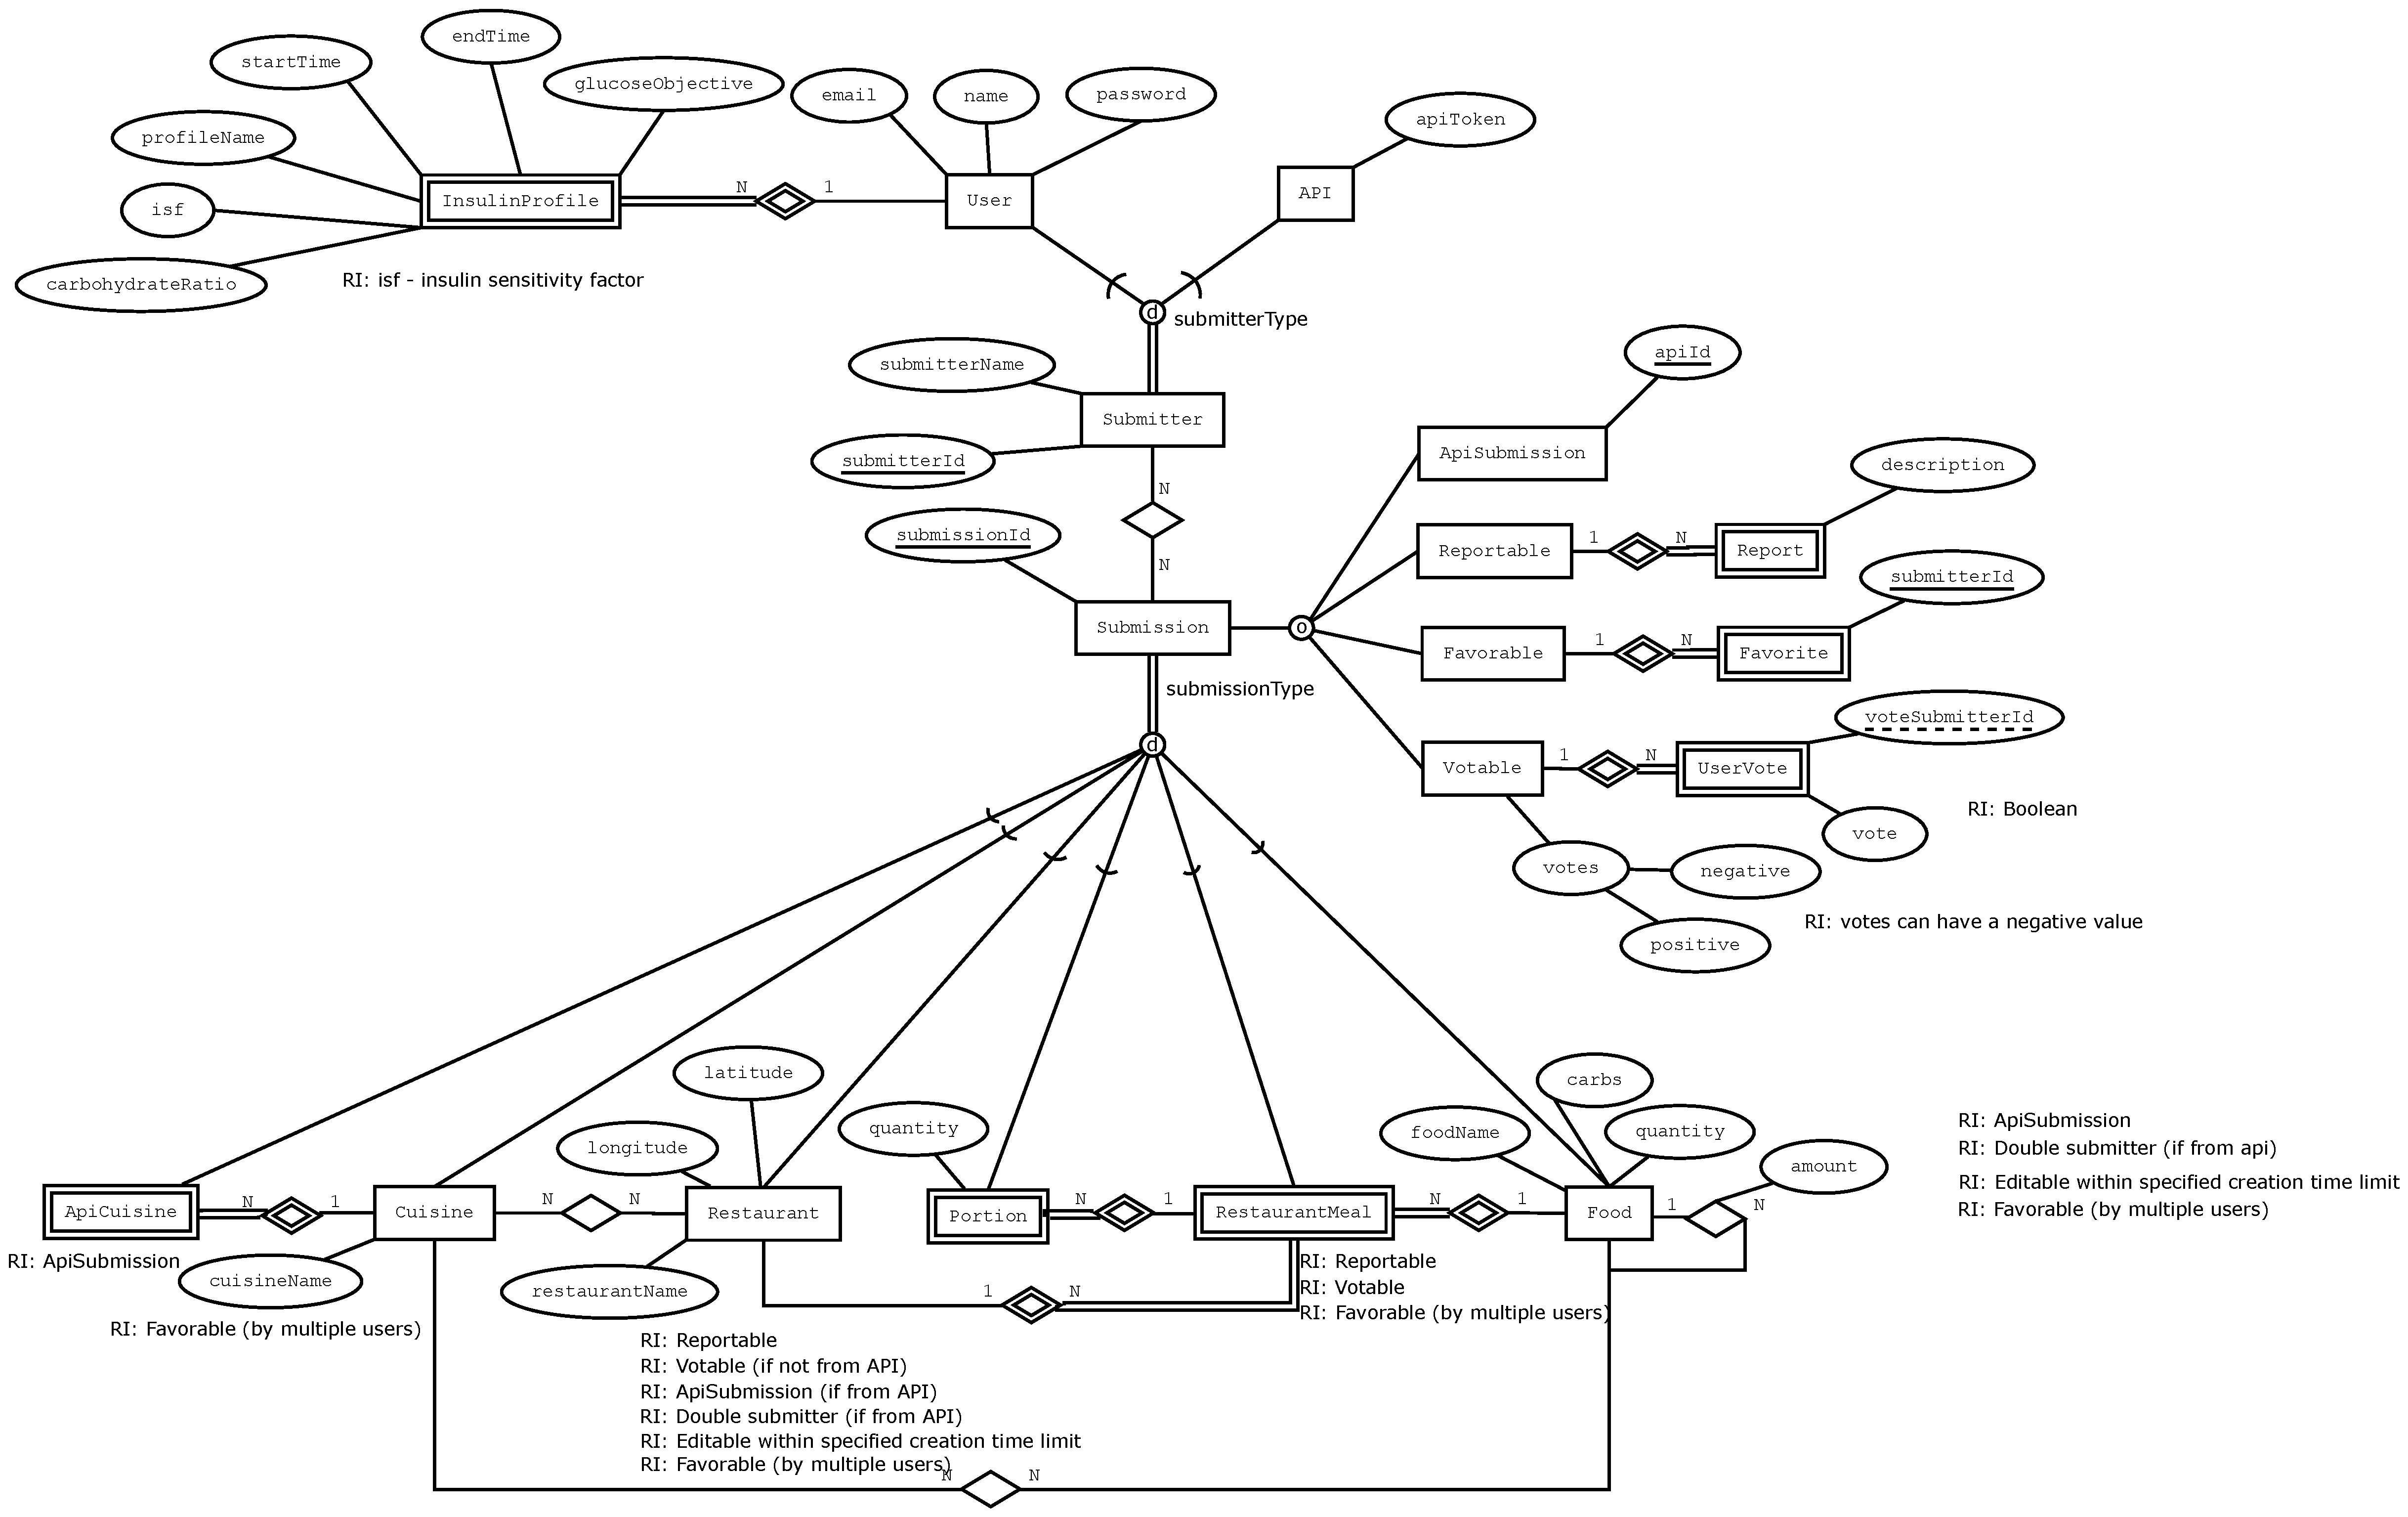
\includegraphics[scale=0.2]{_figures/Nutr.io_Database_Diagram.eps}
    \caption{Database conceptual model}
\end{figure}

The database's relational model is present inside this report's appendix [\nameref{app:relational_model}].\\

In the relational model there are tables which are not specified in the conceptual model.
These are a product from the normalization and associations between entities which will simplify queries' complexity.\\

Now the submission can fall into 4 categories: ApiSubmission, Reportable, Favorable and Votable, in order to disguish between submissions that
are from the user or from APIs and to separate which ones can be reportable, favorable and votable by the user.\\

The cuisine entity has now an associated entity called ApiCuisine, to save cuisine information provided by the Here API.\\

Meals and ingredients were now condensed into one entity called food - now each meal can have meals inside it that can also be considered
ingredients in other contexts.\\

Therefore each meal possesses nutritional information, which is essential to the user especially to the insulin calculations. That information is composed by
'carbs' - meal's carbohydrates; and quantity - meal's quantity.\\

\section{HTTP server}

\subsection{Used tecnologies}

\subsubsection{Kotlin}

We chose to use Kotlin\cite{kotlin} for the HTTP server developed as it is a language that is being more adopted and used nowadays and because it is totally 
interoperable with Java\cite{java}.\\

It was also the language used during PDM, which is an optional course for Android application development inside the LEIC programme, 
making this a language we felt confortable with.\\

\subsubsection{Spring MVC}

At the beginning of the project we decided to use Spring MVC\cite{springmvc} rather than Ktor\cite{ktor}, as the first one is taught in DAW, which is an optional course
for Web applications development inside the LEIC programme. As Spring MVC has a better coverage inside the LEIC programme, we considered 
it a more solid choice.\\

\subsubsection{Used dependencies}

Here are all the dependencies injected inside HTTP server gradle settings file.\\

\begin{itemize}
    \item \textbf{Kotlin base dependencies} - kotlin-reflect and kotlin-stdlib-jdk8;
    \item \textbf{Spring base dependencies} - spring-boot-starter and starter-web;
    \item \textbf{Mockito} - for tests with mocks;
    \item \textbf{Jackson} - for JSON serialization and deserialization;
    \item \textbf{JDBI} - the driver/interface for connecting with the relational database;
    \item \textbf{Spring Security} - for authentication and authorization proposes.
\end{itemize}

\subsection{Code structure}

The HTTP server uses a Spring MVC implementation, structuring its' code in several layers:\\

\begin{itemize}
    \item MVC Controller layer, uses multiple services and handles input to model and model to
     output \textit{DTO} mappings through \textit{DTO} class mappers. Data Transfer Objects (\textit{DTO}):
     For every model there is an equivalent input and output \textit{DTO} class which is represented by its
     corresponding suffix, e.g. "\textit{InsulinProfilesInput}" and "\textit{InsulinProfilesOutput}".
     Controller classes are prefixed by "\textit{Controller}".
     \item Service layer, uses multiple repositories and handles model to database \textit{DTO} and database \textit{DTO}
      to model mapping through instance mappers. The mapper classes used to map the \textit{DTOs} to model have a domain prefix e.g.
      "\textit{Db}" or "\textit{Api}" while having a type "\textit{Mapper}" suffix e.g. "\textit{DbRestaurantMapper}". 
      The service class names are prefixed by "\textit{Service}". 
      \item Data Access layer, is ranged between repositories and Data Access Objects (\textit{DAOs}), each repository
       uses various \textit{DAOs} that represent each database entity/relation through JDBI declarative API. 
       For database \textit{DTOs}, the prefix "\textit{Db}" is used before the table name and then the suffix "\textit{DTO}". For \textit{DAOs} it was used the
       table name and the prefix "\textit{Dao}" e.g. "\textit{UserDao}". Repository classes are
       prefixed by "\textit{Repository}" e.g. "\textit{RestaurantDbRepository}". 
\end{itemize}

\begin{figure}[H]
    \begin{center}
        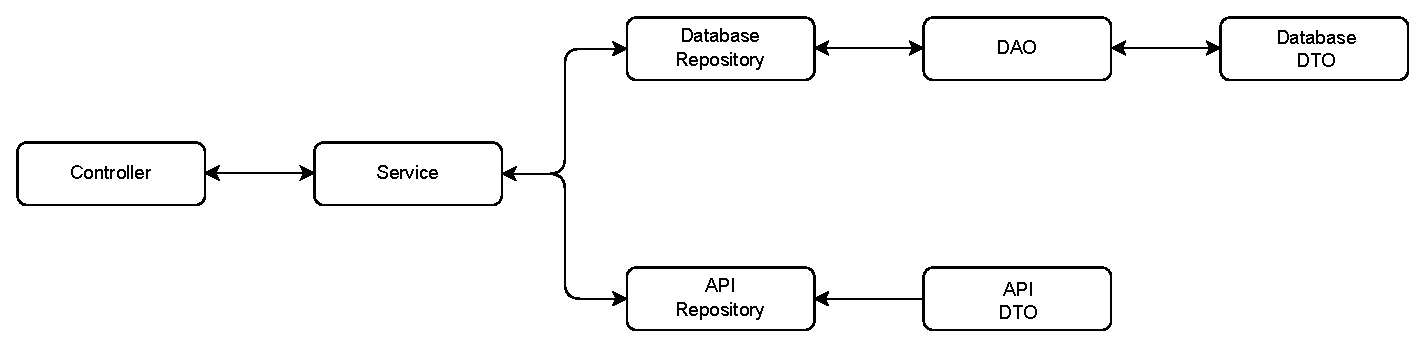
\includegraphics[scale=0.7]{_figures/server-classes.eps}
        \caption{Server's classes structure}
    \end{center}
\end{figure}

\subsection{Routing and endpoints}

\begin{figure}[H]
    \begin{center}
        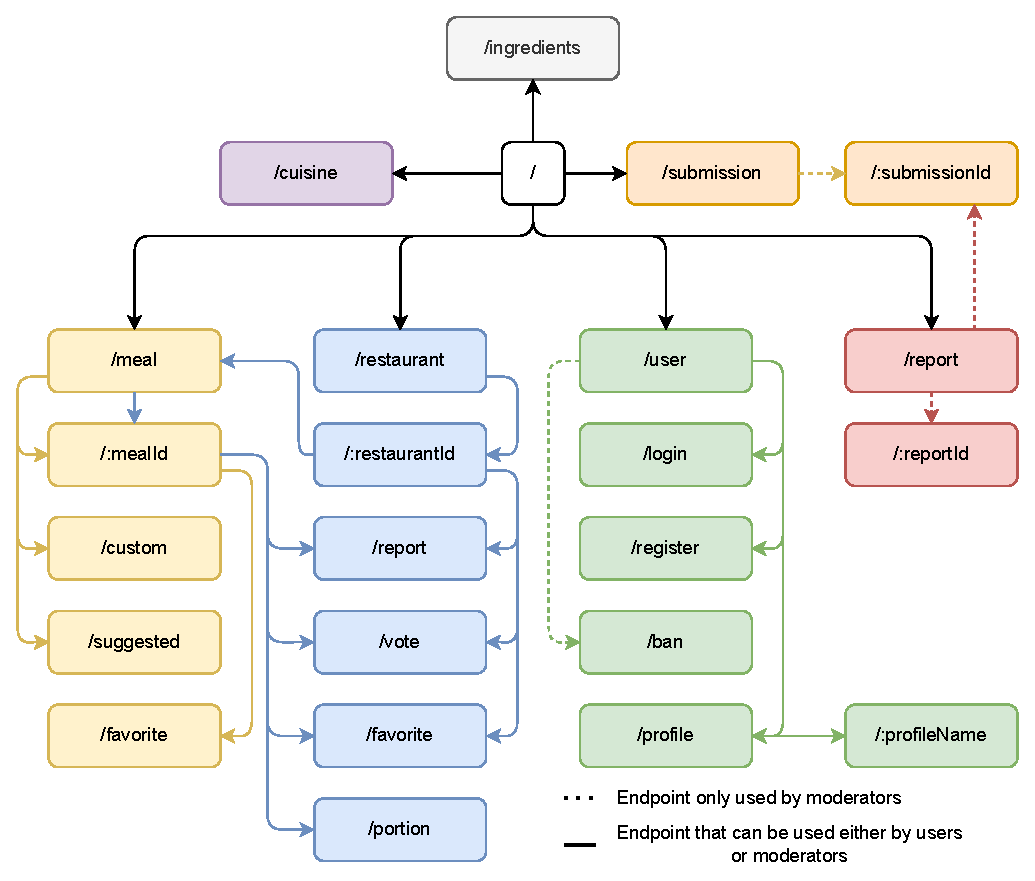
\includegraphics[scale=0.8]{_figures/endpoints_diagram.eps}
        \caption{The server's routing}
    \end{center}
\end{figure}

The picture presented above represents a simplified diagram that shows how the navigation between endpoints occurs.
It should be taken in consideration that, as the picture's label says, some nodes represented in this diagram are used by 
both users and moderators and the diagram can not label those situations with detail. Those details can be better analysed
in this report appendix about endpoints.\\

The color code used in this diagram represents where each endpoint starts providing a better comprehension
and visualization, e.g.: /restaurant/:restaurantId/meal/:mealId (endpoint for a specific restaurant meal) starts with a blue
node (/restaurant); /meal/suggested (endpoint for suggested meals) starts with a yellow node (/meal).\\

\subsection{Kotlin sequences}

As previously stated, Kotlin is completely interoperable with Java and, as such, streams are also supported. However Kotlin introduced sequences which bring
advantages over Java streams. In this subsection it will be presented the reasons why we chose sequences over streams during development.

\subsubsection{Performance}

There are 3 main aspects that affect the performance overhead of sequences and streams:
 \begin{itemize}
     \item \textbf{Primitive handling}: Sequences include methods which simplify common actions and thus avoid primitive values autoboxing, even if sequences don't have primitive variants like streams.
     \item \textbf{Optional values}: Streams create optional wrappers when values might not be present, while sequences use nullable types, being more efficient by not creating optional wrappers.
     \item \textbf{Lambda creation}: Sequences create fewer lambda instances than streams, resulting in more efficiency.
 \end{itemize}

 \subsubsection{Simplicity}

 Sequences have more specialized actions and functions making the code more simple and easy to read.

 \subsubsection{Null safety}

 Sequences use Kotlin nullable types so safe usage is enforced at compile time, being safer from a null safety prespective. It becomes more efficient as streams force Optional-wrapping of values which are not present.

 \subsubsection{Overall}

 \textbf{Stream advantages}
 \begin{itemize}
     \item Have primitive variants to avoid unnecessary autoboxing;
     \item Enables easy parallelism via parallel streams.
 \end{itemize}

 \textbf{Sequence advantages}
 \begin{itemize}
     \item Don’t introduce platform types;
     \item Use compile-time null-safety and scale well with safe-call and Elvis operators;
     \item Are shorter due to fewer operations;
     \item Simpler aggregates;
     \item Simpler terminal operations;
     \item Don’t create wrapper objects for values that might be missing;
     \item Create fewer lambda instances and most terminal operations are inlined resulting in improved efficiency;
 \end{itemize}


\subsection{Request lifecycle}
Each request is received in a spring controller mapping, with input object,
parameters or path variables as arguments. When receiving an input object \textit{DTO},
it will be validated with java's \textit{javax.validation} (Hibernate).
Once validated the input model's data might be used in subsequent service layer calls.\\

Repositories are used on the service level to handle all \textit{DAO} interactions with
the database and other HTTP API requests. The resulting responses (input and database \textit{DTOs})
are converted to the model \textit{DTOs} according to their response mappers.
All API calls are made from asynchronous HTTP requests, while database calls block the calling thread.\\

\subsection{JDBI}

After some discussion of which driver should be used to allow communication between the server and database, we decided that the JDBI\cite{jdbi} was the best
option as it is a library built on JDBC\cite{jdbc}.\\

The library also exposes two different API's styles: a fluent/imperative style and a declarative style (used during development), as shown below.

\begin{figure}[H]
    \begin{center}
        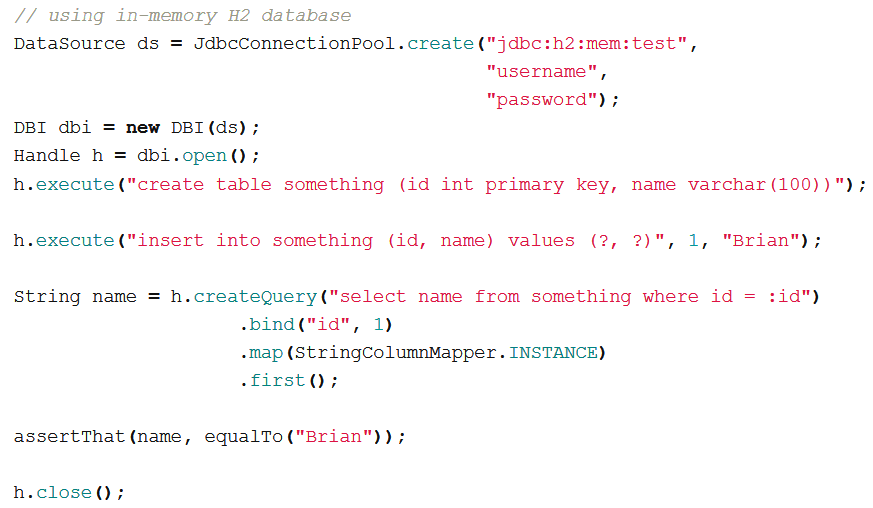
\includegraphics[scale=0.5]{_figures/fluentApiJdbi.png}
        \caption{JDBI using an imperative API style}
    \end{center}
\end{figure}

\begin{figure}[H]
    \begin{center}
        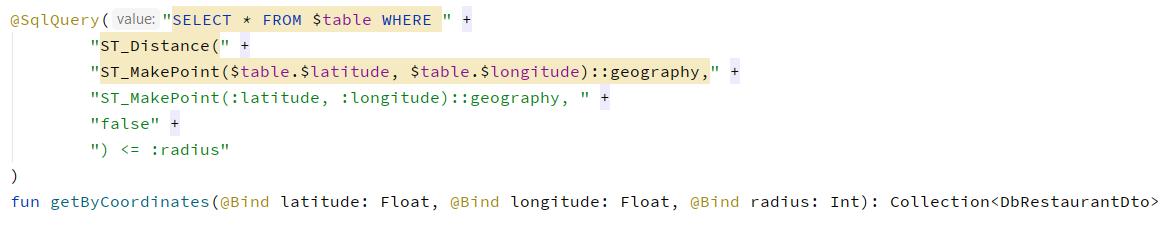
\includegraphics[scale=0.5]{_figures/sqlObjectJdbi.png}
        \caption{JDBI using a declarative API style (example from HTTP server)}
    \end{center}
\end{figure}

We chose to use a declarative style due to its convenience and code simplicity
over the imperative one. It was also the more adequate style to the project's structure. 

\subsection{Spring Security}

\subsubsection{JSON Web Tokens}

As each client needs to have authentication to provide the user a way to create an account and allow submissions and data synchronization,
we had to discuss about the platform's security and the safest ways to do that.\\

It was concluded that the use of \textbf{JSON Web Tokens}\cite{jwt} was the best option, because of the nature of the clients, more specifically the fact that
the mobile application is completely \textbf{stateless}.\\

Another advantage is the fact that these tokens have an expiration time, which means that after a certain amount of time they are no longer valid.
In case of security breach, this feature becomes useful, because if a valid token is stolen, neither the attacker has a way to generate valid tokens 
nor does he know the user's password. The token could only be used by a short period of time (10h), easing the amount of damage that an intruder can
make and confining it to only one user inside the platform.\\

The picture below represents a very generic and simplified workflow of the JSON Web Token. 

\begin{figure}[H]
    \begin{center}
        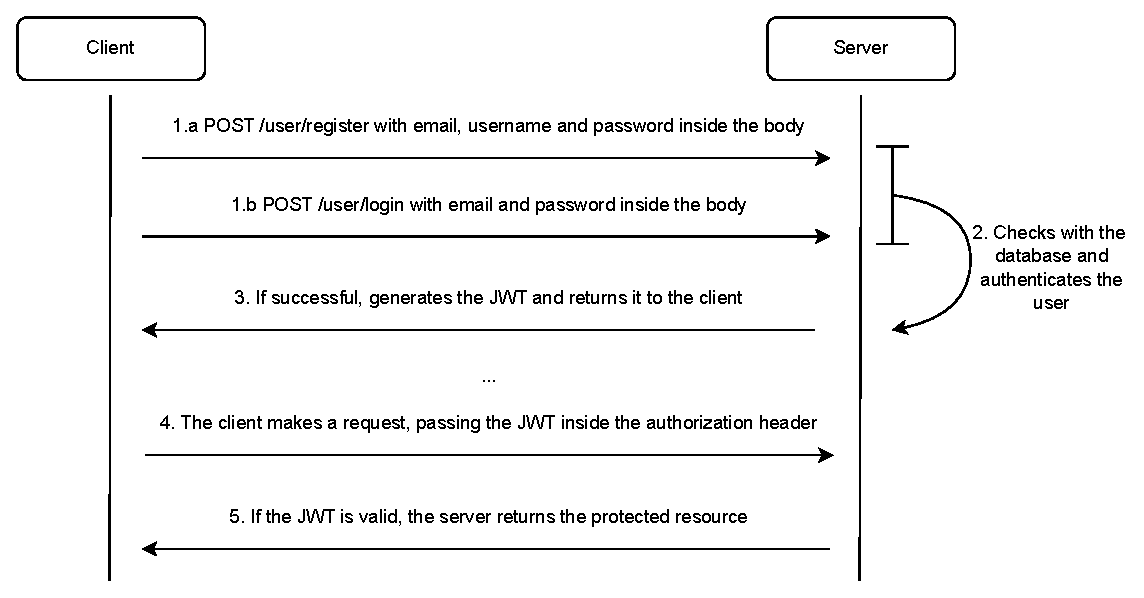
\includegraphics[scale=0.9]{_figures/JWT-simple-diagram.eps}
        \caption{The JWT workflow}
    \end{center}
\end{figure}

\subsubsection{Implementation}

To implement the shown workflow inside the HTTP server, as we are implementing it with Spring, the more obvious choice was to use \textbf{Spring Security}\cite{springsecurity}.\\

Spring Security is a customizable authentication and access-control framework.\\

The picture below shows how the server handles an user login using this framework.\\

\newpage
\begin{figure}[H]
    \begin{center}
        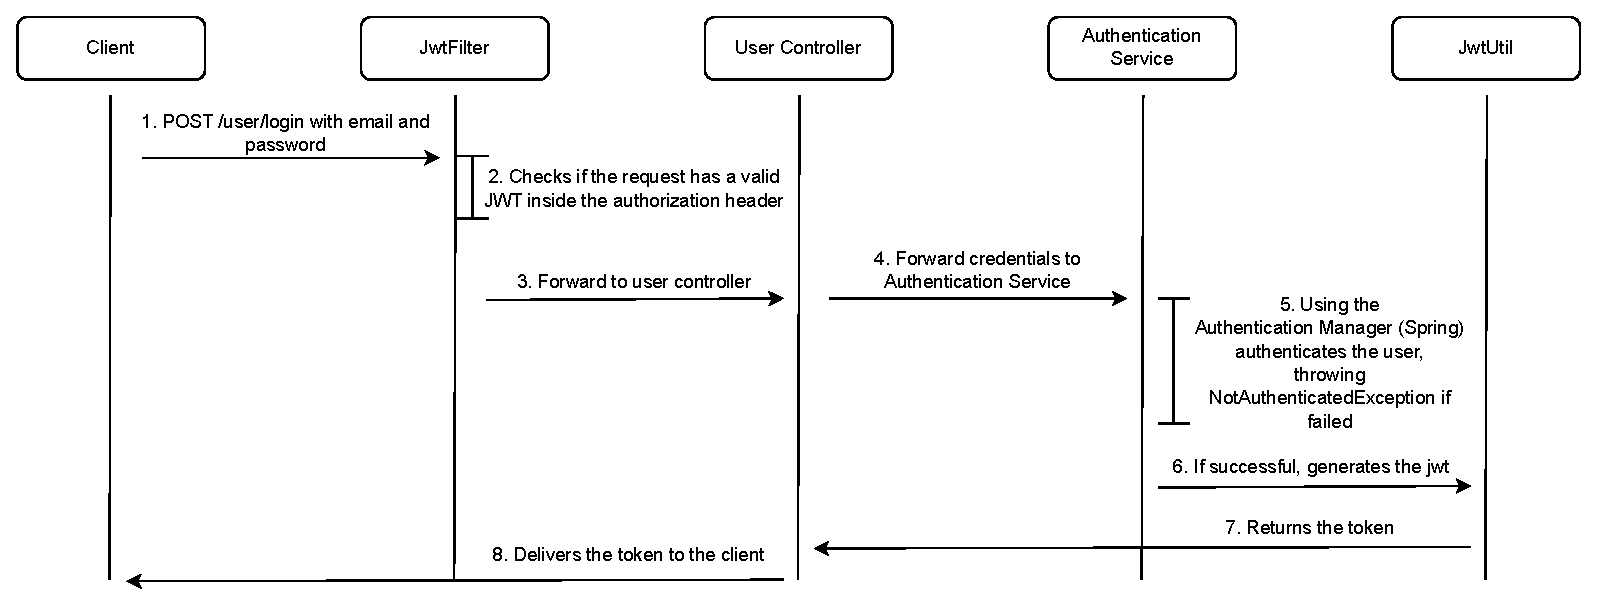
\includegraphics[scale=0.60]{_figures/Spring-jwt-diagram.eps}
        \caption{A Spring security workflow example with the POST /user/login}
    \end{center}
\end{figure}

After the previously mentioned dependencies are installed, the WebSecurityConfig is the first class to be constructed. Here are specified, via antMatchers, which
endpoints do not need authentication, acting like a whitelist, so every endpoint that is not specified via antMatchers needs authentication, and will return code 401
Unauthorized if the JWT is invalid. The JWT filter is also started up inside this class.\\

The UserAuthenticationArgumentResolver class, as the name says, is an argument resolver that filters each request, acting before it reaches the desired controller,
checking the authentication header and extracting the jwt from the Bearer verifying if it is valid.\\

The Authentication service class calls the Spring Authentication Manager and authenticates the user, it provides methods which call the JwtUtil
to retrieve the email from the token or encode the password when registering.\\

The password encoding always happens when the user registers for the first time: the server hashes the password using \textbf{BCrypt}\cite{bcrypt} before inserting the new
user into the database.\\

BCrypt is a password-hashing function based on the Blowfish\cite{blowfish} cipher. We found this function very convenient for these reasons:
\begin{itemize}
    \item Already pre salts the passwords, preventing rainbow table attacks\cite{rainbowtable};
    \item Makes bruteforce attacks inviable: the iteration count can be increased to make it even slower to crack.
    This cipher makes even GPU-powered bruteforce attacks impracticable due to this feature.
\end{itemize}

The JwtUtil is the core class which validates, generates and adds claims to the tokens.\\

\subsubsection{User data safety}

In the previous section it was shown that the user can register an account. It was made this way so the server can store
insulin profiles, which will be better explained in the mobile application's section. The insulin profiles store user sensitive
information and are encrypted when written inside the database using a symmetric cipher (AES-256) with a private key provided by an 
environment variable from the host machine.\\

The user can also delete its account. When an account is deleted all user sensitive information is deleted from the server: email,
username, password, insulin profile and custom meals. However, its submitter identifier, which is a database generated number,
is maintained in order to preserve its public submissions, in order to keep the platform's data consistent, so a user that makes many 
public insertions does not compromise our data's consistency if its account is deleted.\\

\section{Geolocation}

Given how all clients rely on obtaining nearby restaurants, there was a need to implement a geolocation function in the project's design.\\

Initial research showcased two possible solutions: Haversine\cite{haversine} distances and cartesian distances, where the latter returns a highly imprecise distances.
As such, Haversine was selected.\\

The next step was to choose which system filters nearby restaurants: database or HTTP server. After some discussion, we decided that database was the best
option for two reasons: 
\begin{itemize}
    \item Given the large amount of existing restaurants, sending such data from the database to the HTTP server so that it could filter it would occupy too much memory;
    \item PostgreSQL already supplies extensions that add support for location queries, namely PostGIS.
\end{itemize}

\section{Android application}

\subsection{Used tecnologies}

\subsubsection{Kotlin}

We chose to use Kotlin for the mobile application development, as it is now the official programming language for Android development,
according to Google.\\

It is also the language taught during the optinal course - mobile devices programming (PDM).\\

\subsubsection{External dependencies}

Here are the dependencies that were included in the mobile application which gave more functionalities to it.

\begin{itemize}
    \item \textbf{Volley} - an HTTP library for Android networking;
    \item \textbf{Jackson} - JSON serialization, deserialization and handling;
    \item \textbf{Room} - A framework to store data locally;
    \item \textbf{MapBox} - A framework to provide maps and geolocation tools;
    \item \textbf{MPAndroidChart} - provides custom graphs inside the application;
    \item \textbf{Glide} - a framework for image loading;
    \item \textbf{Androidx crypto} - a new crypto library made by Google, used to encrypt User credentials.
\end{itemize}

\subsection{Code structure}

\subsubsection{Drawing pattern}

The mobile application code structure follows the \textbf{repository pattern}, which is a code architecture recommended by the \textbf{Android Jetpack}\cite{jetpack} for this type of applications.\\

\begin{figure}[H]
    \begin{center}
        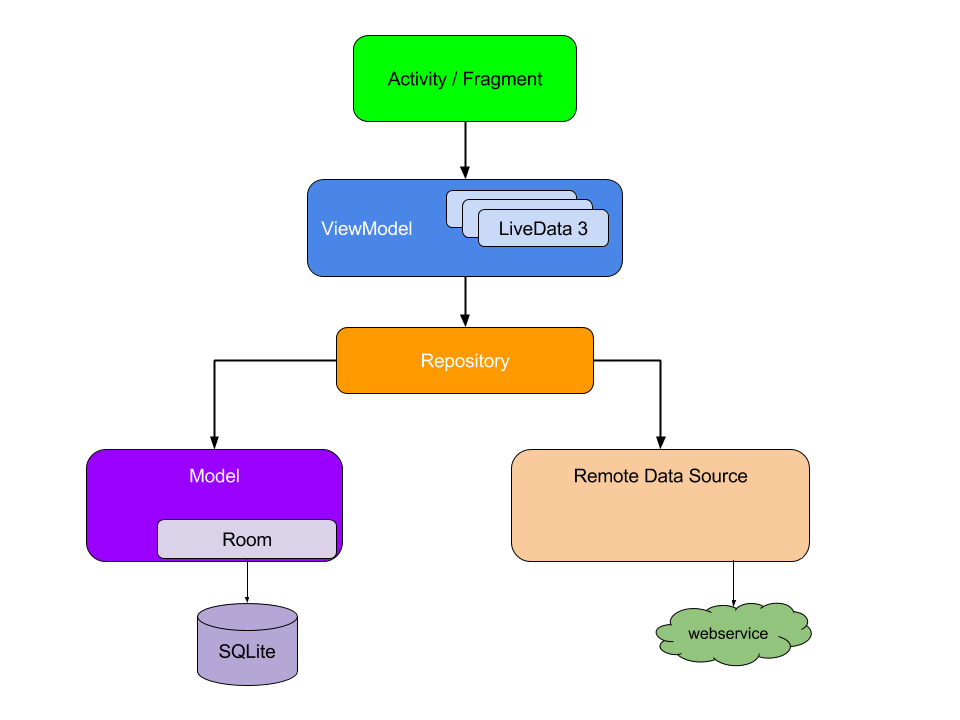
\includegraphics[scale=0.5]{_figures/repository_pattern2.png}
        \caption{The repository pattern diagram}
    \end{center}
\end{figure}

Above there is the pattern's diagram provided by the Android Jetpack.\\

The idea behind this architecture is that each Activity or fragment has its own ViewModel and each one calls the needed functions present inside the repository.
The repository is a layer that manages where the information should be retrieved from.\\

The 'DTO to model' mapping also occurs inside the repository, following the rule where ViewModels should only manipulate models and the layers below should only use DTOs.\\

By following this pattern, the code becomes segmented and organized, allowing a good comprehension and code maintainability.\\

Just as the server the android client has the input and output "\textit{DTOs}" suffixed with "\textit{input}" and "\textit{output}". 
These classes are mapped by input mappers prefixed with "\textit{input}".\\

The Activity, Fragments, ViewModel, Adapters and Repositories classes are all prefixed by their type.

\subsubsection{Fragments}

We chose to use fragments\cite{fragment} for each application view instead of activities. Although a fragment has a more complex lifecycle than the activity and depends on it
to exist, they are far more lightweight to instanciate than an activity and thus they provide more performance to the application.\\ 

It is also the recommended Android widget to use when designing an application with a side drawer.\\

\subsubsection{Modular interfaces}

As the code in the mobile application development became repetitive, the group decided to implement modular interfaces,
which are interfaces that can be implemented by fragments and viewholders and provide them predefined behaviours.

\subsection{Local data storing}

As mentioned in the dependencies, the mobile application utilizes Room to store data locally. This is convenient
for multiple reasons: 
\begin{itemize}
    \item To allow using the application in offline situations;
    \item To save data in order to avoid unnecessary requests to the server;
    \item To help data synchronization, that will be detailed later in this section.
\end{itemize}

Room classes use the "\textit{Db}" prefixed followed by the name and prefixed by their type e.g. "\textit{DbMealInfoMapper}", "\textit{DbMealInfoRelation}" and "\textit{DbMealInfoEntity}". 
The \textit{DAO} classes However are only prefixed with "\textit{Dao}". 
All entities are mapped by a database mapper suffixed with "\textit{Mapper}".

\subsection{User authentication and authorization}

The user has the ability to register and login in the mobile application. Besides being the server responsable for these functions, the mobile application has also some intervention
here, because after a successful login or register, the HTTP server will return a jwt (JSON Web Token) that will authenticate and authorize the user in future requests.\\

This token will be stored in the Android Shared Preferences\cite{sharedpreferences} and it will also to be renewed periodically due to its 10h expiration time. The user credentials will also be saved
inside the mobile device to allow automatic logins to renew the user's JSON Web Token and avoid its expiration.\\

\subsubsection{Problem: The content inside the shared preferences is written in plaintext. Is it safe to store user credentials inside the shared preferences?}

Although the Android Shared Preferences being a safe place to store application information, this fact is not completely true:
a normal device can not access these preferences and it should be a safe place to store user credentials, however rooted devices\cite{root} can easily
access the shared preferences file and retrieve plaintext from it, which would compromise the user security.\\

\subsubsection{Resolution: Androidx Crypto}

The Androidx crypto\cite{crypto} was used to solve this issue. This library is used to encrypt the user credentials before writing them inside the mobile device.\\

These new Google library takes advantage of the Android KeyStore\cite{keystore} system, which encrypts information using a hardware-level encryption, making the
encryption even harder to break. The information is encrypted using a symmetric cipher algorithm (AES-256), the key used to sign and encrypt information
is hardware-generated and it is managed by the application itself, so the key's retrieval from an 'encrypted' shared preferences is equal to the 'normal'
shared preferences.\\

We also discussed if the credentials should be saved inside the device or if only the database should possess them.
If that approach was taken, the user had to login each time it was needed to read or write a protected resource.\\

As this platform is not, for example, a bank application that needs top protection. We found this level of protection
unnecessary for the application and inconvenient for the user and decided that only the essential protection should be provided - 
user credentials encryption to avoid information leaks from rooted devices.

\subsection{Data synchronization}

Background data synchronization will happen after a successful login or register. The only user data that will be synchronized are:
\begin{itemize}
    \item Insulin profiles;
    \item Custom meals made by the user;
    \item Favorites.
\end{itemize}

When logged in, the data can be synchronized in two ways:
\begin{itemize}
    \item the user forces the synchronization by swiping down on a list;
    \item The Android WorkManager will make sure that the data is synchronized at least once a 
    day when the phone is inactive and connected to the internet.    
\end{itemize}

\subsection{Android version compatibility}

In order to garantee a global support by most of the Android devices nowadays, the mobile application is supported since \textbf{Android 7} (API level 24)
up to \textbf{Android 10} (API level 29).

\subsection{Functionalities}

Here will be displayed pictures of the mobile application and its functionalities.\\

\subsubsection{Register and Login}

\begin{figure}[H]
    \captionsetup[subfigure]{justification=centering}
    \begin{center}
        \begin{subfigure}{.3\textwidth}
            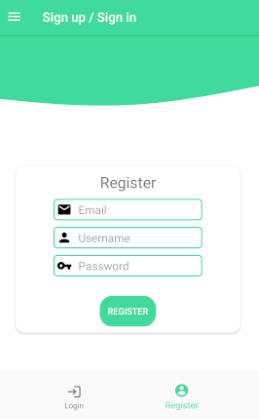
\includegraphics[scale=0.1, width=\textwidth]{_figures/register.png}
            \caption{The register fragment} 
        \end{subfigure}
        \begin{subfigure}{.3\textwidth}
            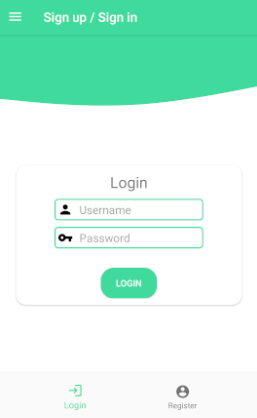
\includegraphics[scale=0.1, width=\textwidth]{_figures/login.png}
            \caption{The login fragment} 
        \end{subfigure}%
        \begin{subfigure}{.3\textwidth}
            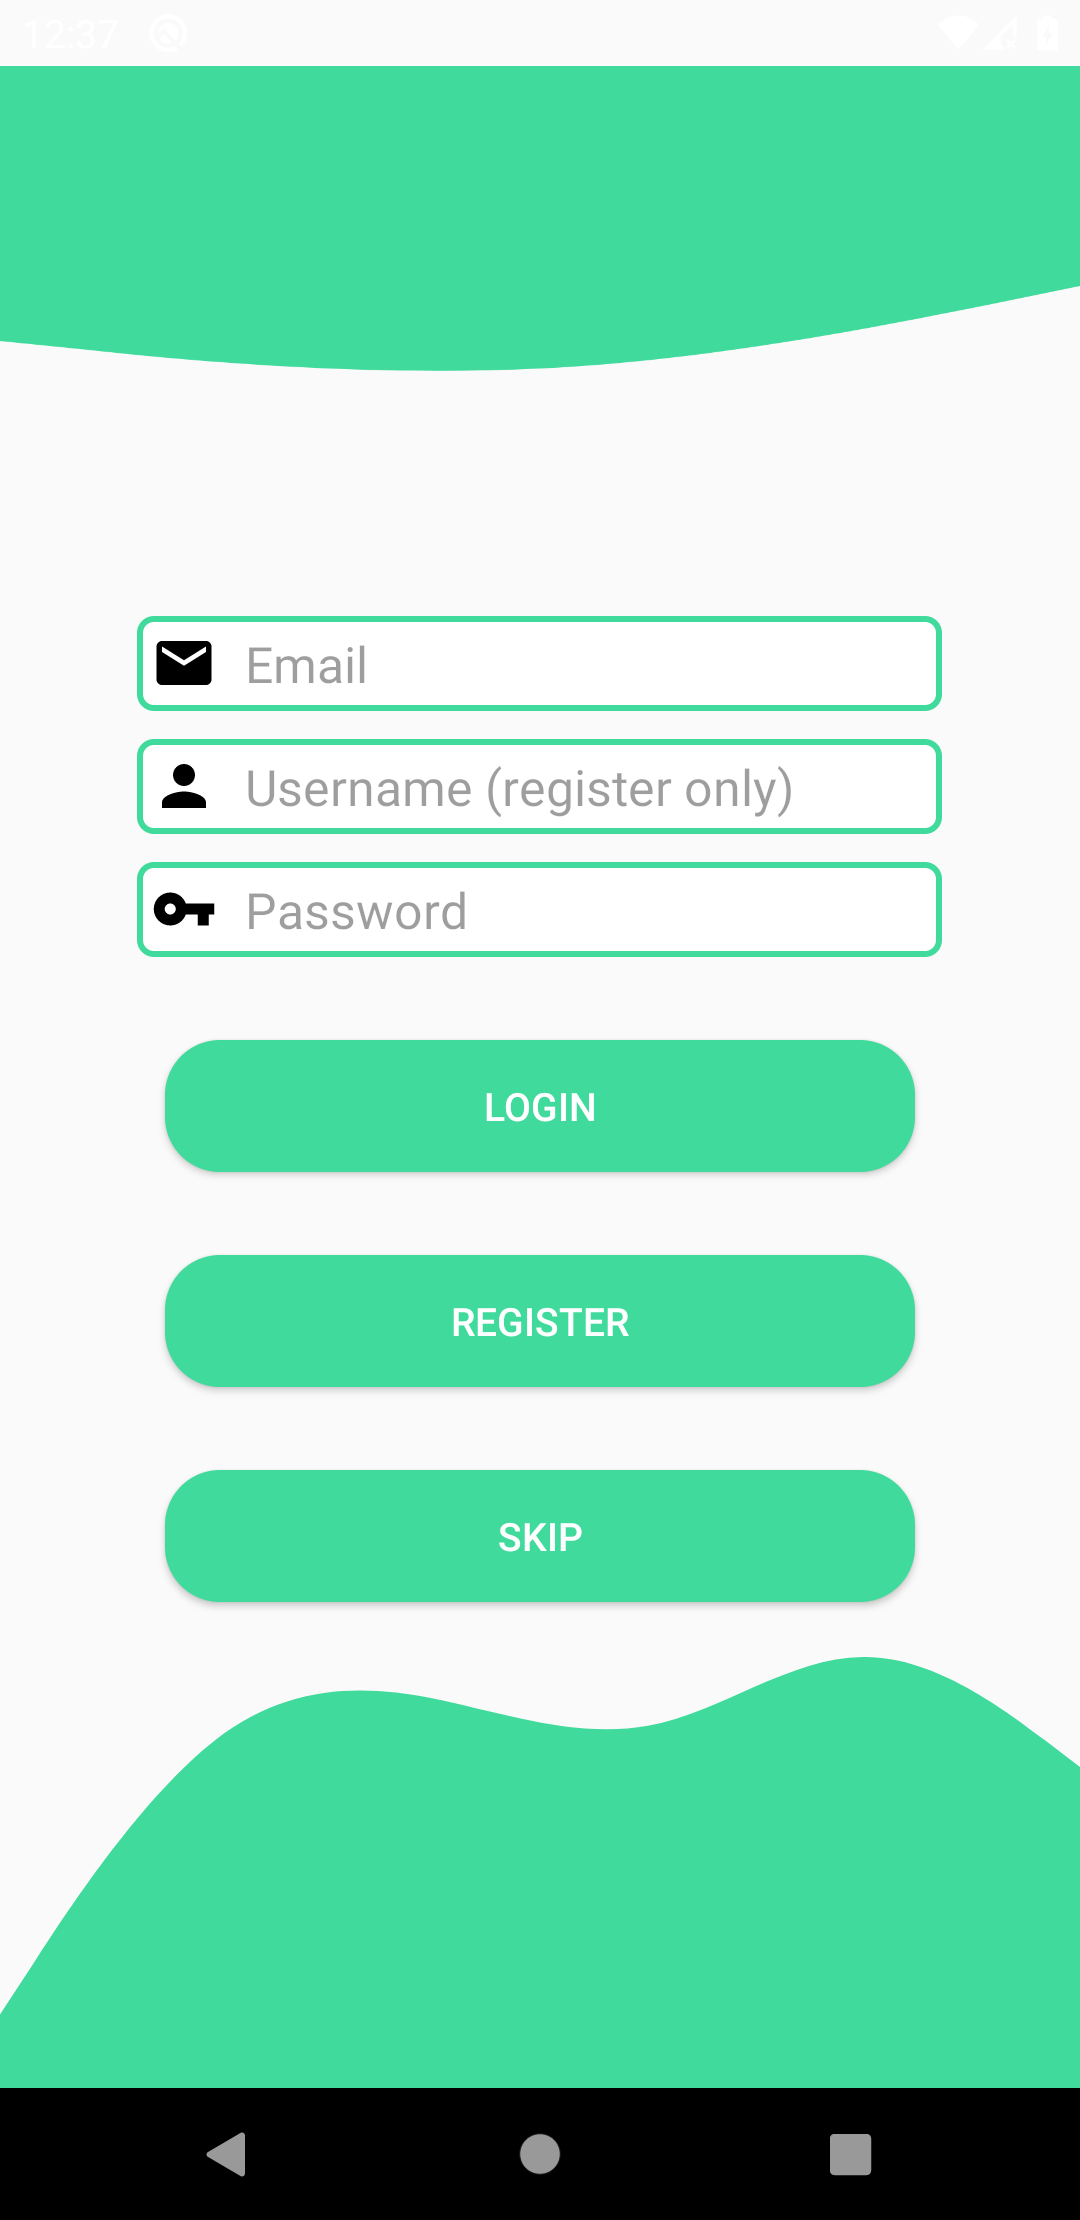
\includegraphics[scale=0.1, width=\textwidth]{_figures/firstSign.png}
            \caption{The sign in/up at the application's startup} 
        \end{subfigure}%
    \end{center}
\end{figure}

Here are the 3 ways a user can register or login inside the mobile application: either on the application's startup or by clicking on the user's profile picture inside the
drawer menu and accessing the slide screen with the bottom bar.\\

Here's the login and register workflow:

\begin{figure}[H]
    \begin{center}
        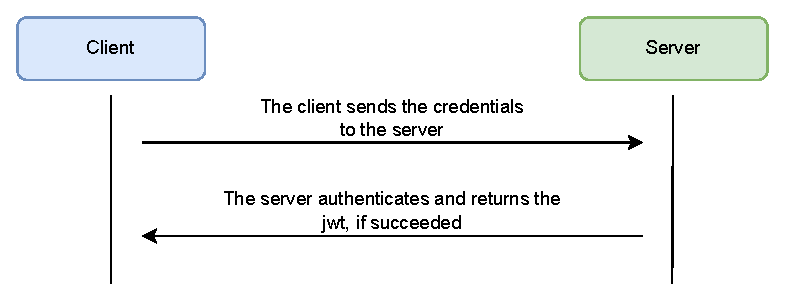
\includegraphics[scale=1]{_figures/auth-workflow.eps}
        \caption{Login and register workflow}
    \end{center}
\end{figure}

\subsubsection{Account deletion}

If the user goes to the login or register fragment again after being successfully logged in, it will see the fragment presented below.

\begin{figure}[H]
    \centering
    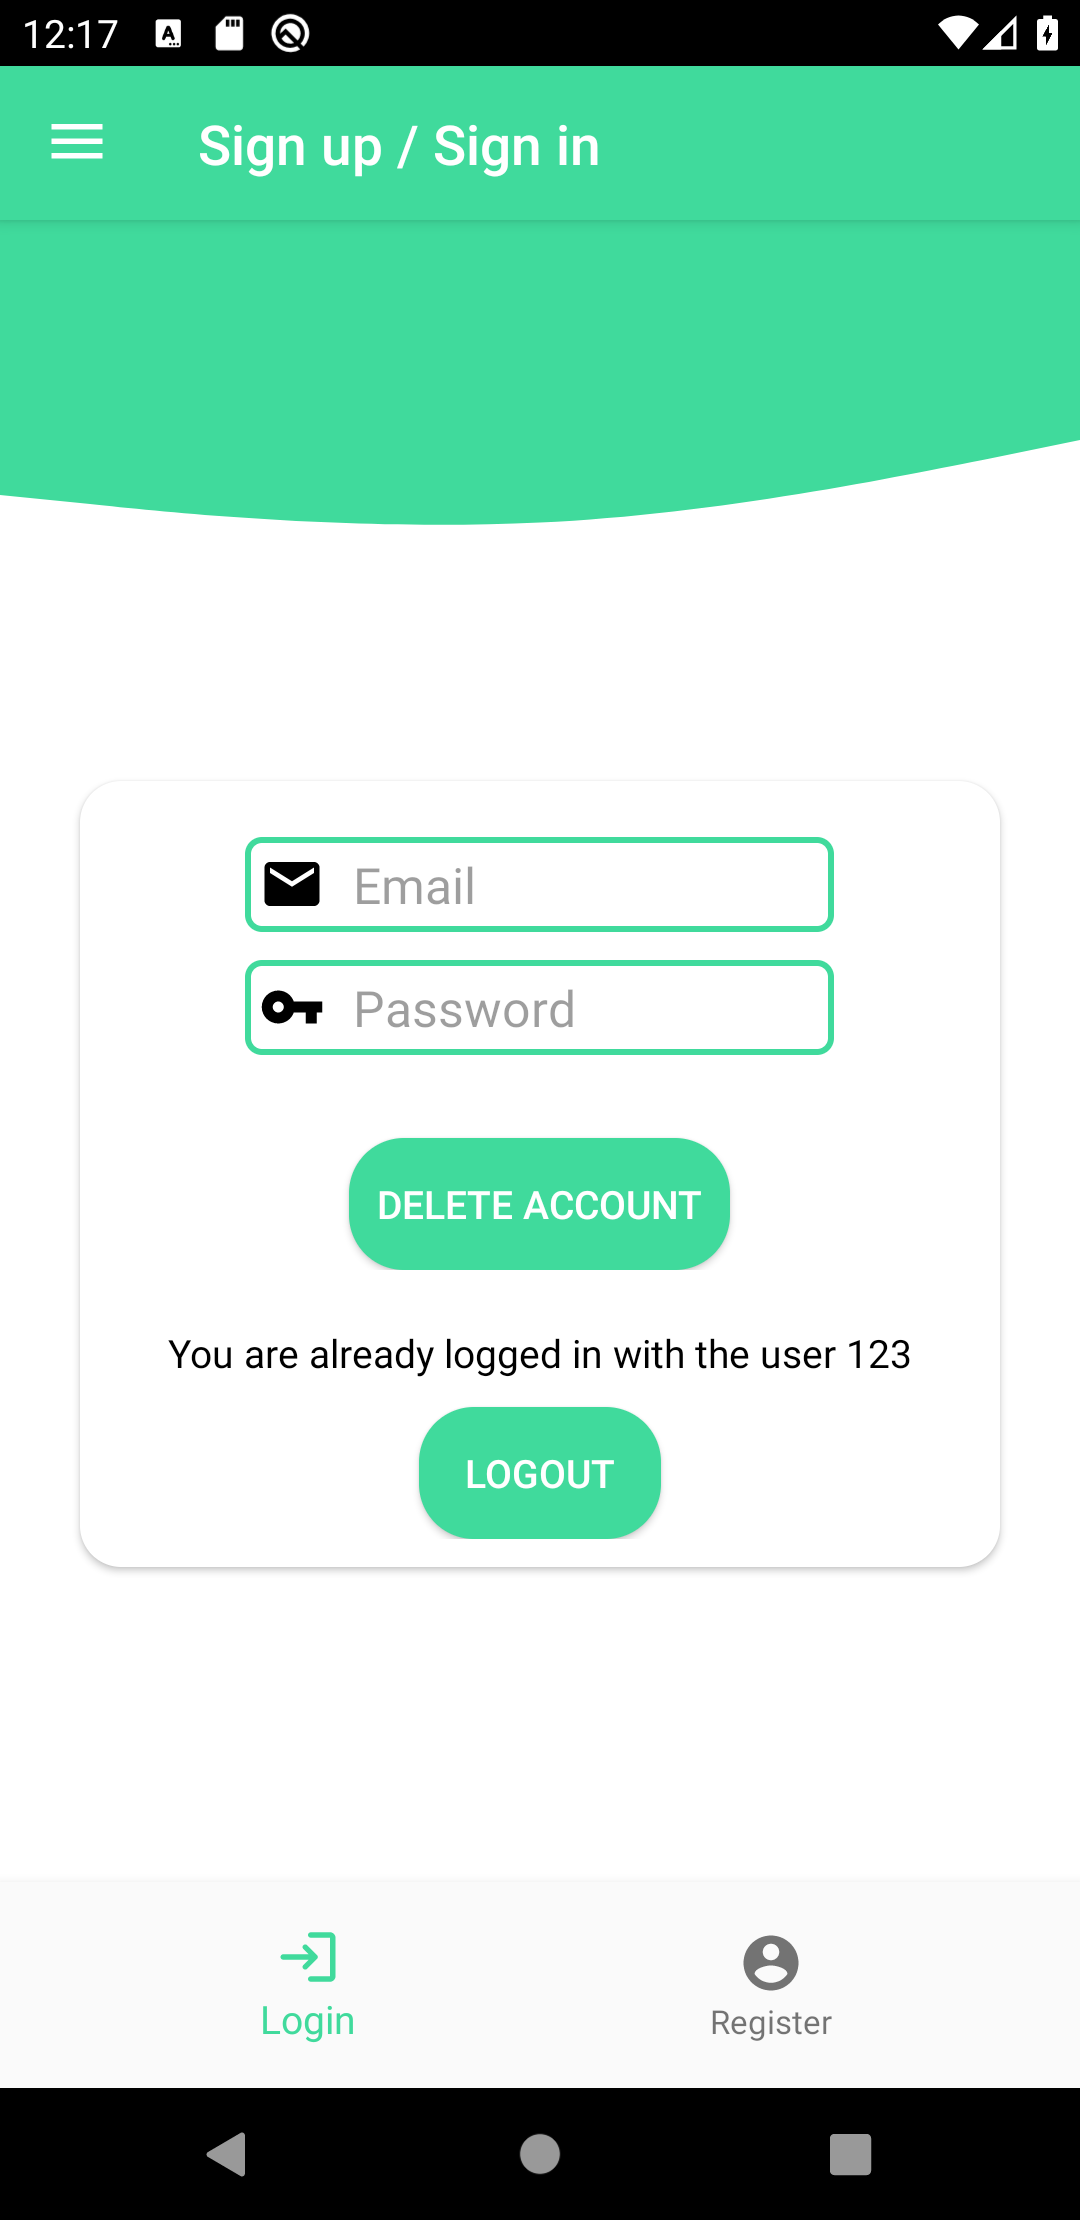
\includegraphics[scale=0.12]{_figures/logout_fragment.png}
    \caption{The register fragment}
\end{figure}

In order to delete the account, the user needs to fill the shown form again and then press the delete account button.\\

After that, the operation will occur as the diagram presented below.

\begin{figure}[H]
    \begin{center}
        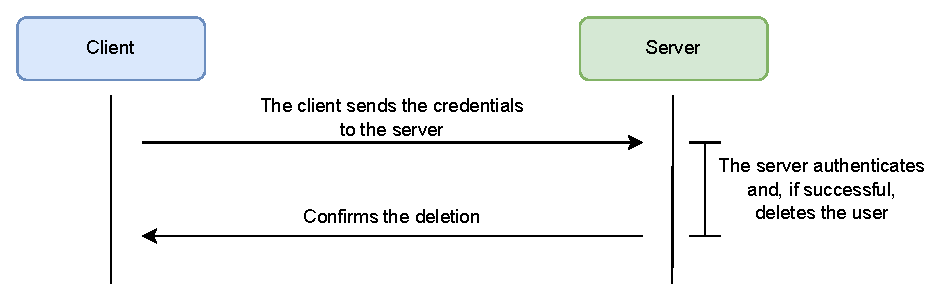
\includegraphics[scale=1]{_figures/user-deletion-workflow.eps}
        \caption{User account deletion workflow}
    \end{center}
\end{figure}

After this only the submitter identifier will remain in database to preserve public submission and all sensitive data
will be deleted.

\subsubsection{Insulin profiles' creation and access}

\begin{figure}[H]
    \captionsetup[subfigure]{justification=centering}
    \begin{center}
        \begin{subfigure}{.3\textwidth}
            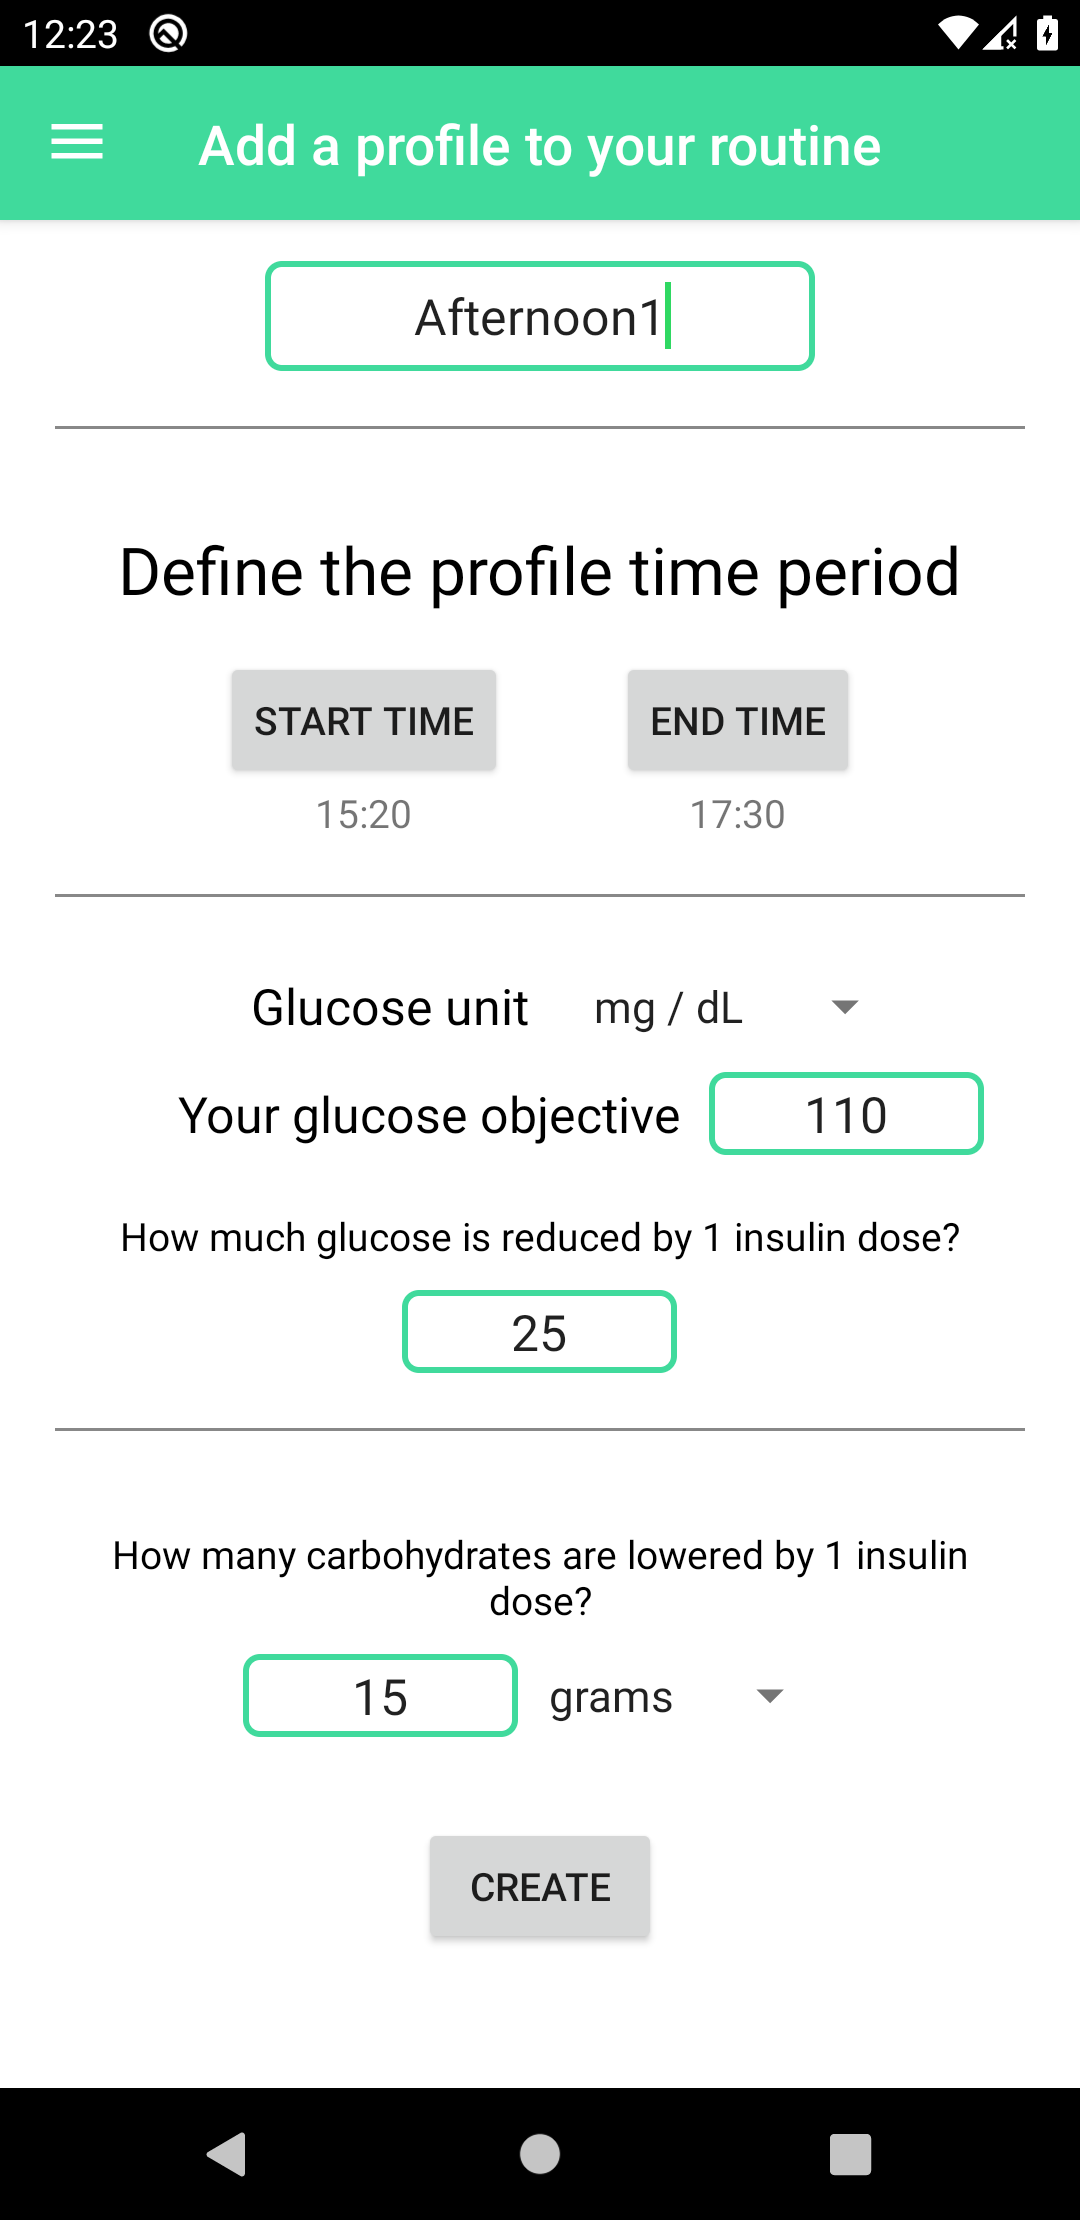
\includegraphics[scale=0.1, width=\textwidth]{_figures/addProfile.png}
            \caption{The fragment to add an insulin profile} 
        \end{subfigure}
        \begin{subfigure}{.3\textwidth}
            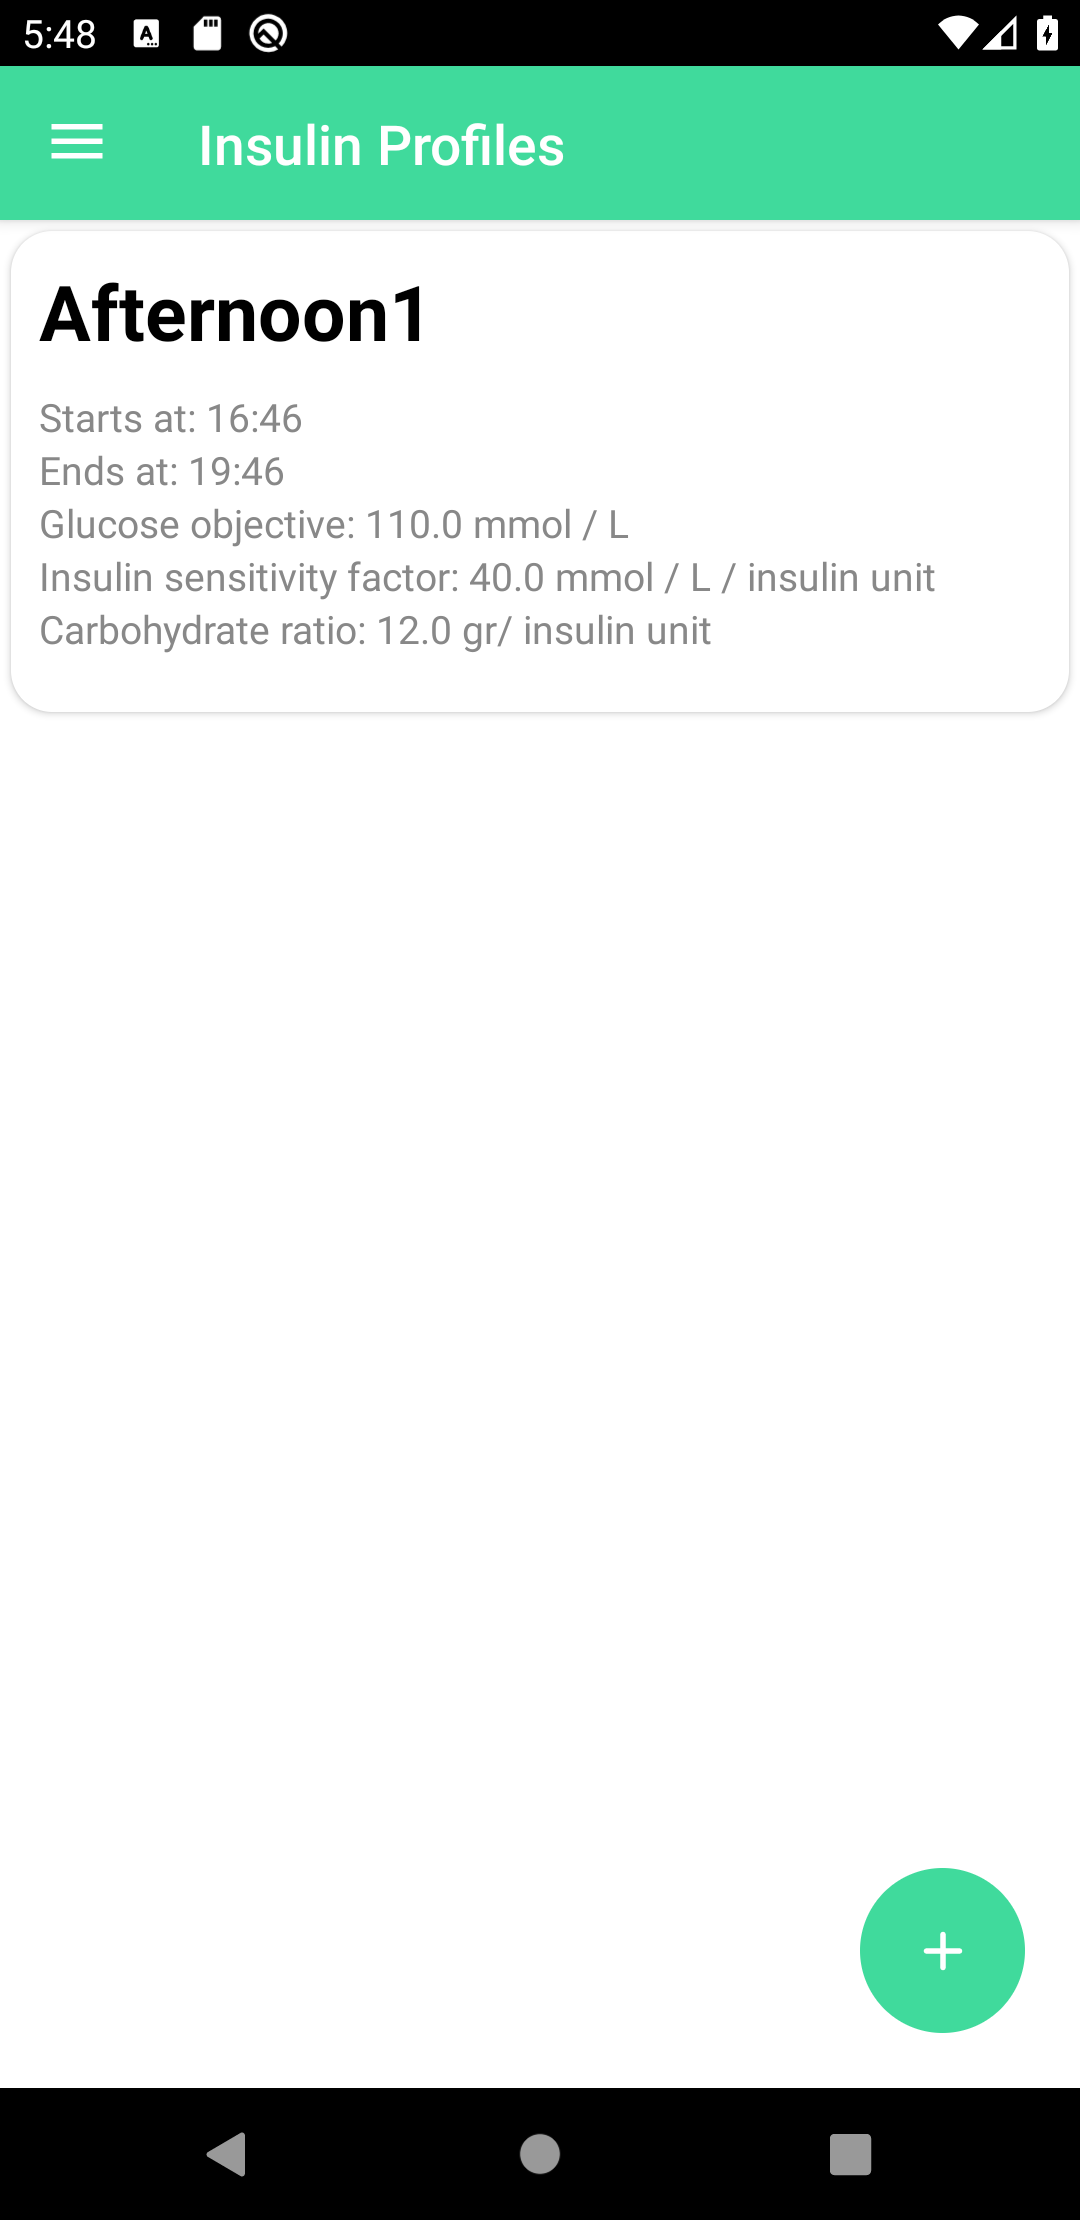
\includegraphics[scale=0.1, width=\textwidth]{_figures/insulin_profiles_list.png}
            \caption{The fragment to access and create insulin profiles} 
        \end{subfigure}
    \end{center}
\end{figure}

The user can map its day with insulin profiles, specifying for a certain timespan its glucose objective, insulin sensitivity and carbohydrates sensitivity, as this parameters
change along the day.\\

When creating insulin profiles, the user must know that a profile's time period can not overlap another and that the time mapping must be done from 00h00 to 23h59, meaning that
the end time can not be before the start time.

\subsubsection{Searching for restaurants and meals}

The user can search for restaurant in two ways:
\begin{itemize}
    \item By accessing 'Map view' inside the Restaurant Box, which will display a list of nearby restaurants along with a map;
    \item By accessing 'By name' inside the Restaurant Box, which will only display a list of restaurants which are also based
    on geolocation.
\end{itemize}

\begin{figure}[H]
    \captionsetup[subfigure]{justification=centering}
    \begin{center}
        \begin{subfigure}{.3\textwidth}
            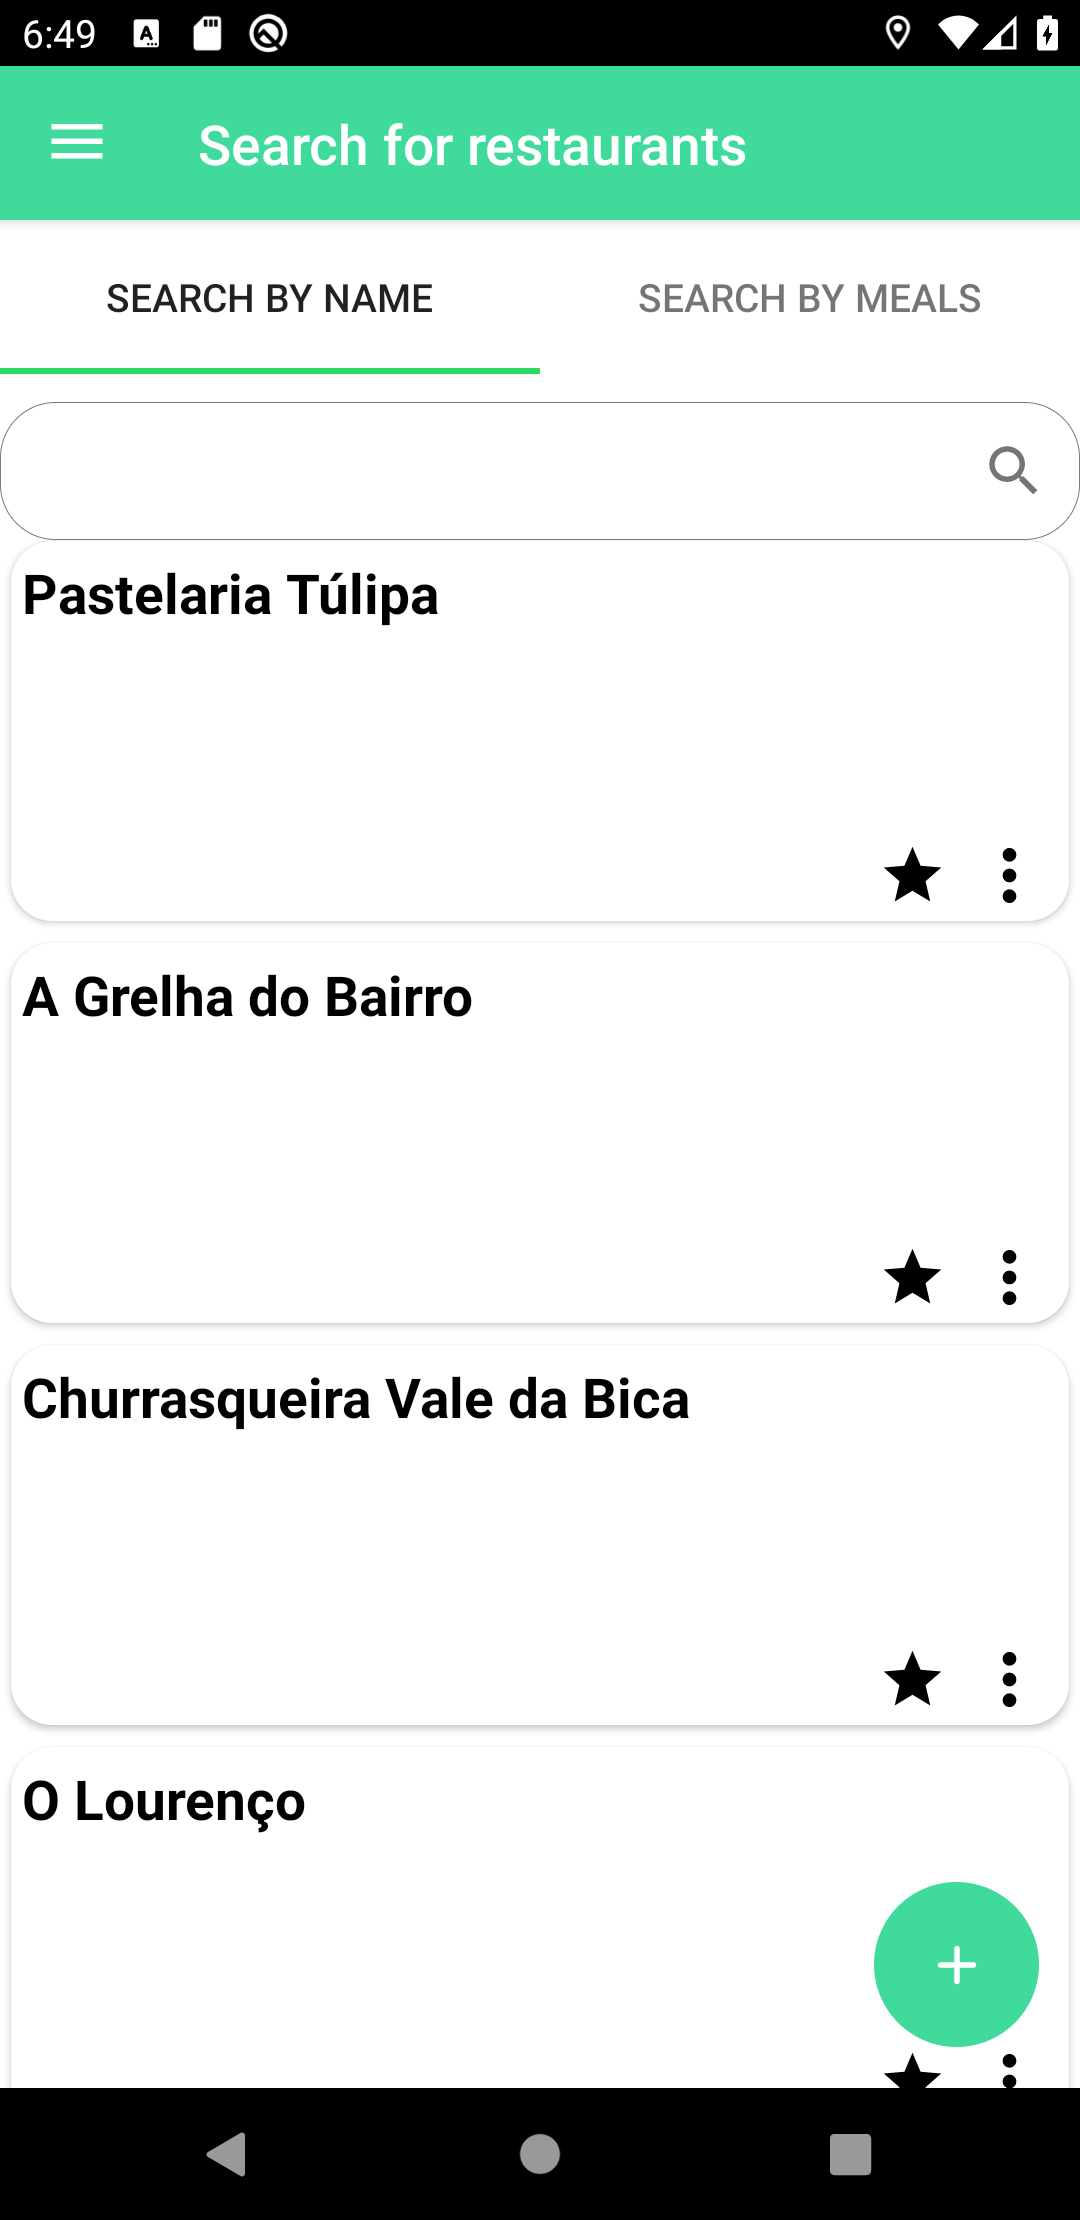
\includegraphics[scale=0.1, width=\textwidth]{_figures/restaurants_by_name.png}
            \caption{Restaurants by location} 
        \end{subfigure}
        \begin{subfigure}{.3\textwidth}
            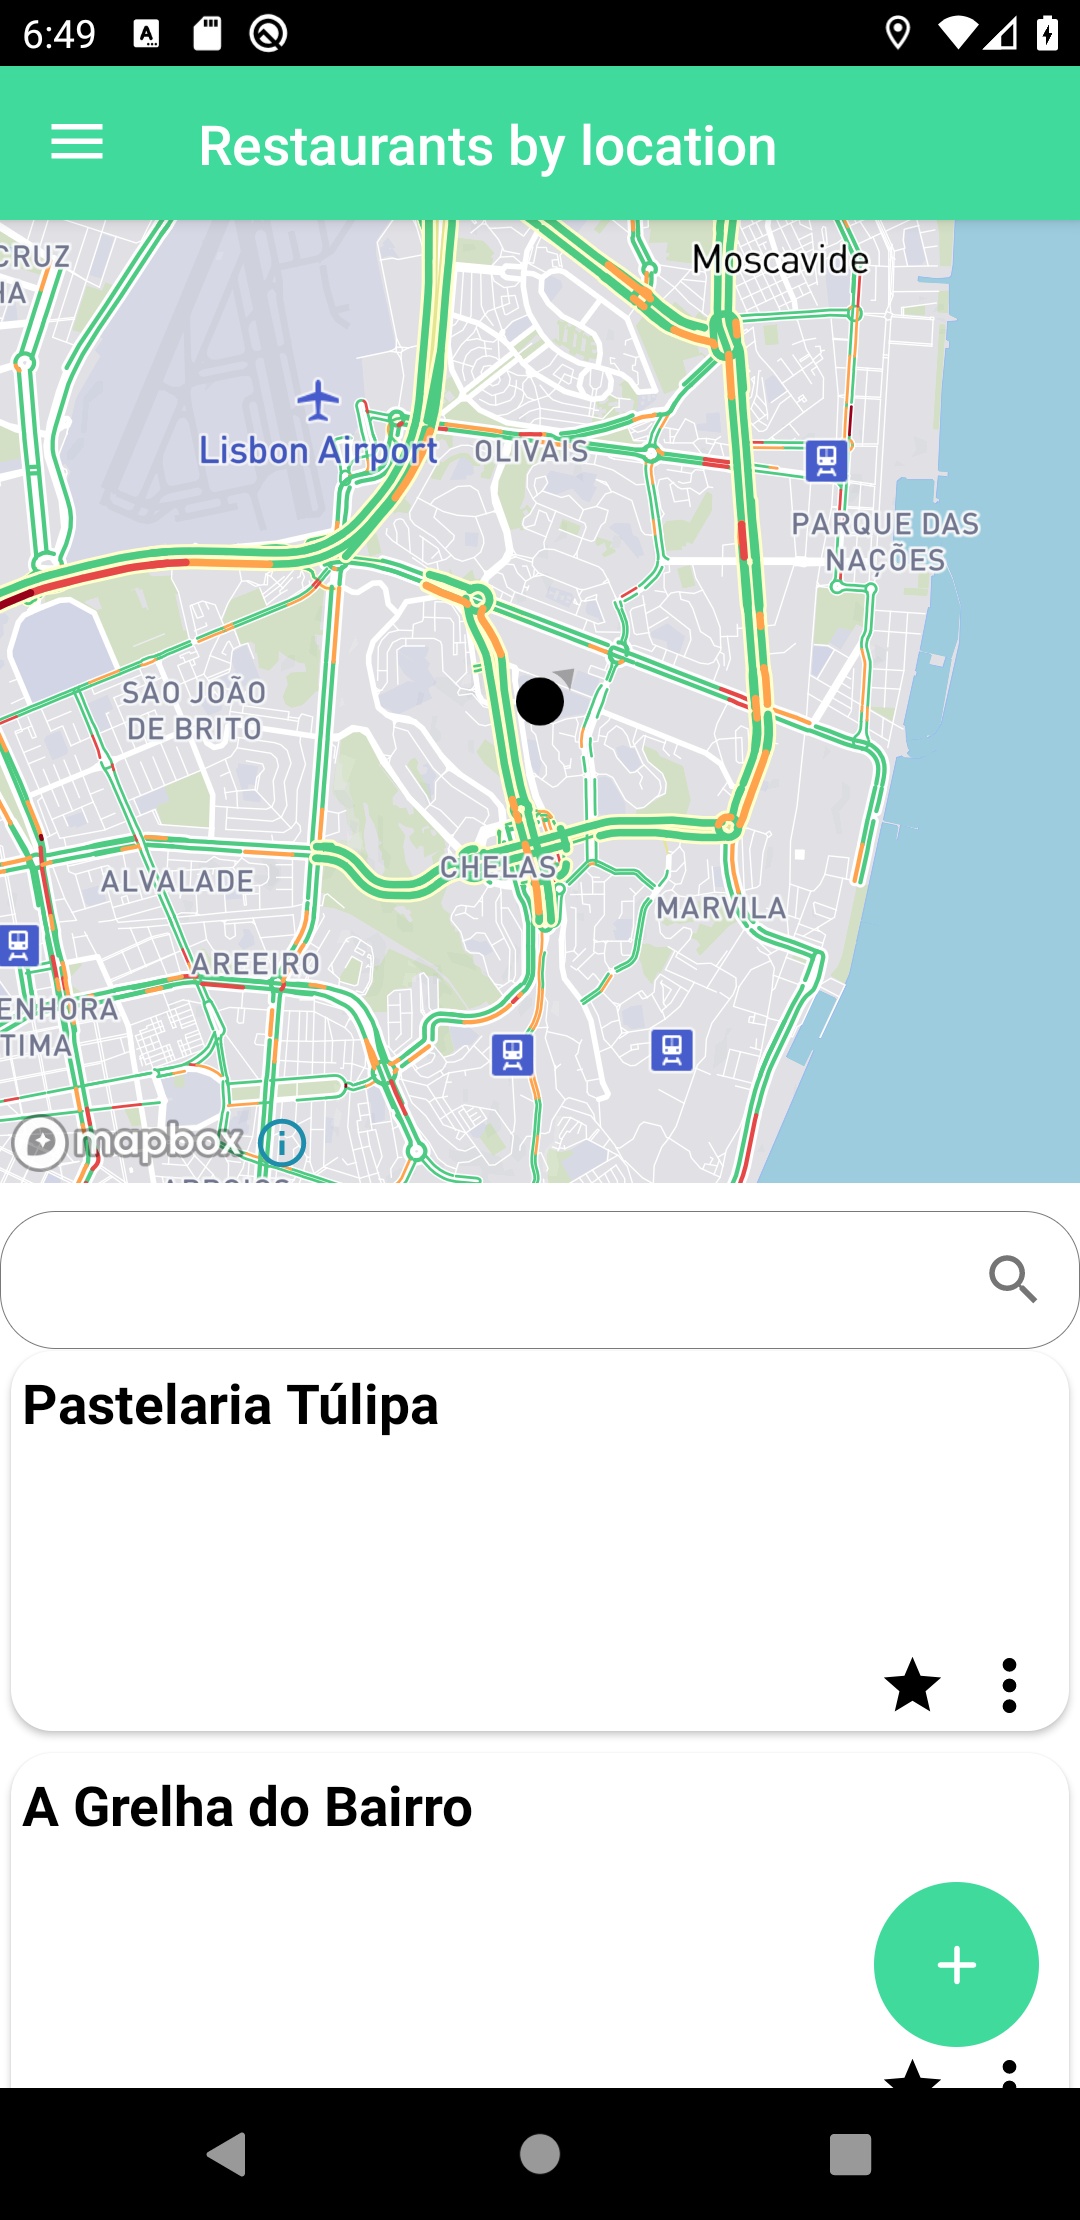
\includegraphics[scale=0.1, width=\textwidth]{_figures/restaurants_map.png}
            \caption{Restaurants by location with map} 
        \end{subfigure}%        
    \end{center}
\end{figure}

The user can also access available meals by accessing 'By name' inside the Meals box, which will display a tab menu with the
platform's suggested meals and meals' ingredients.

\begin{figure}[H]
    \captionsetup[subfigure]{justification=centering}
    \begin{center}
        \begin{subfigure}{.3\textwidth}
            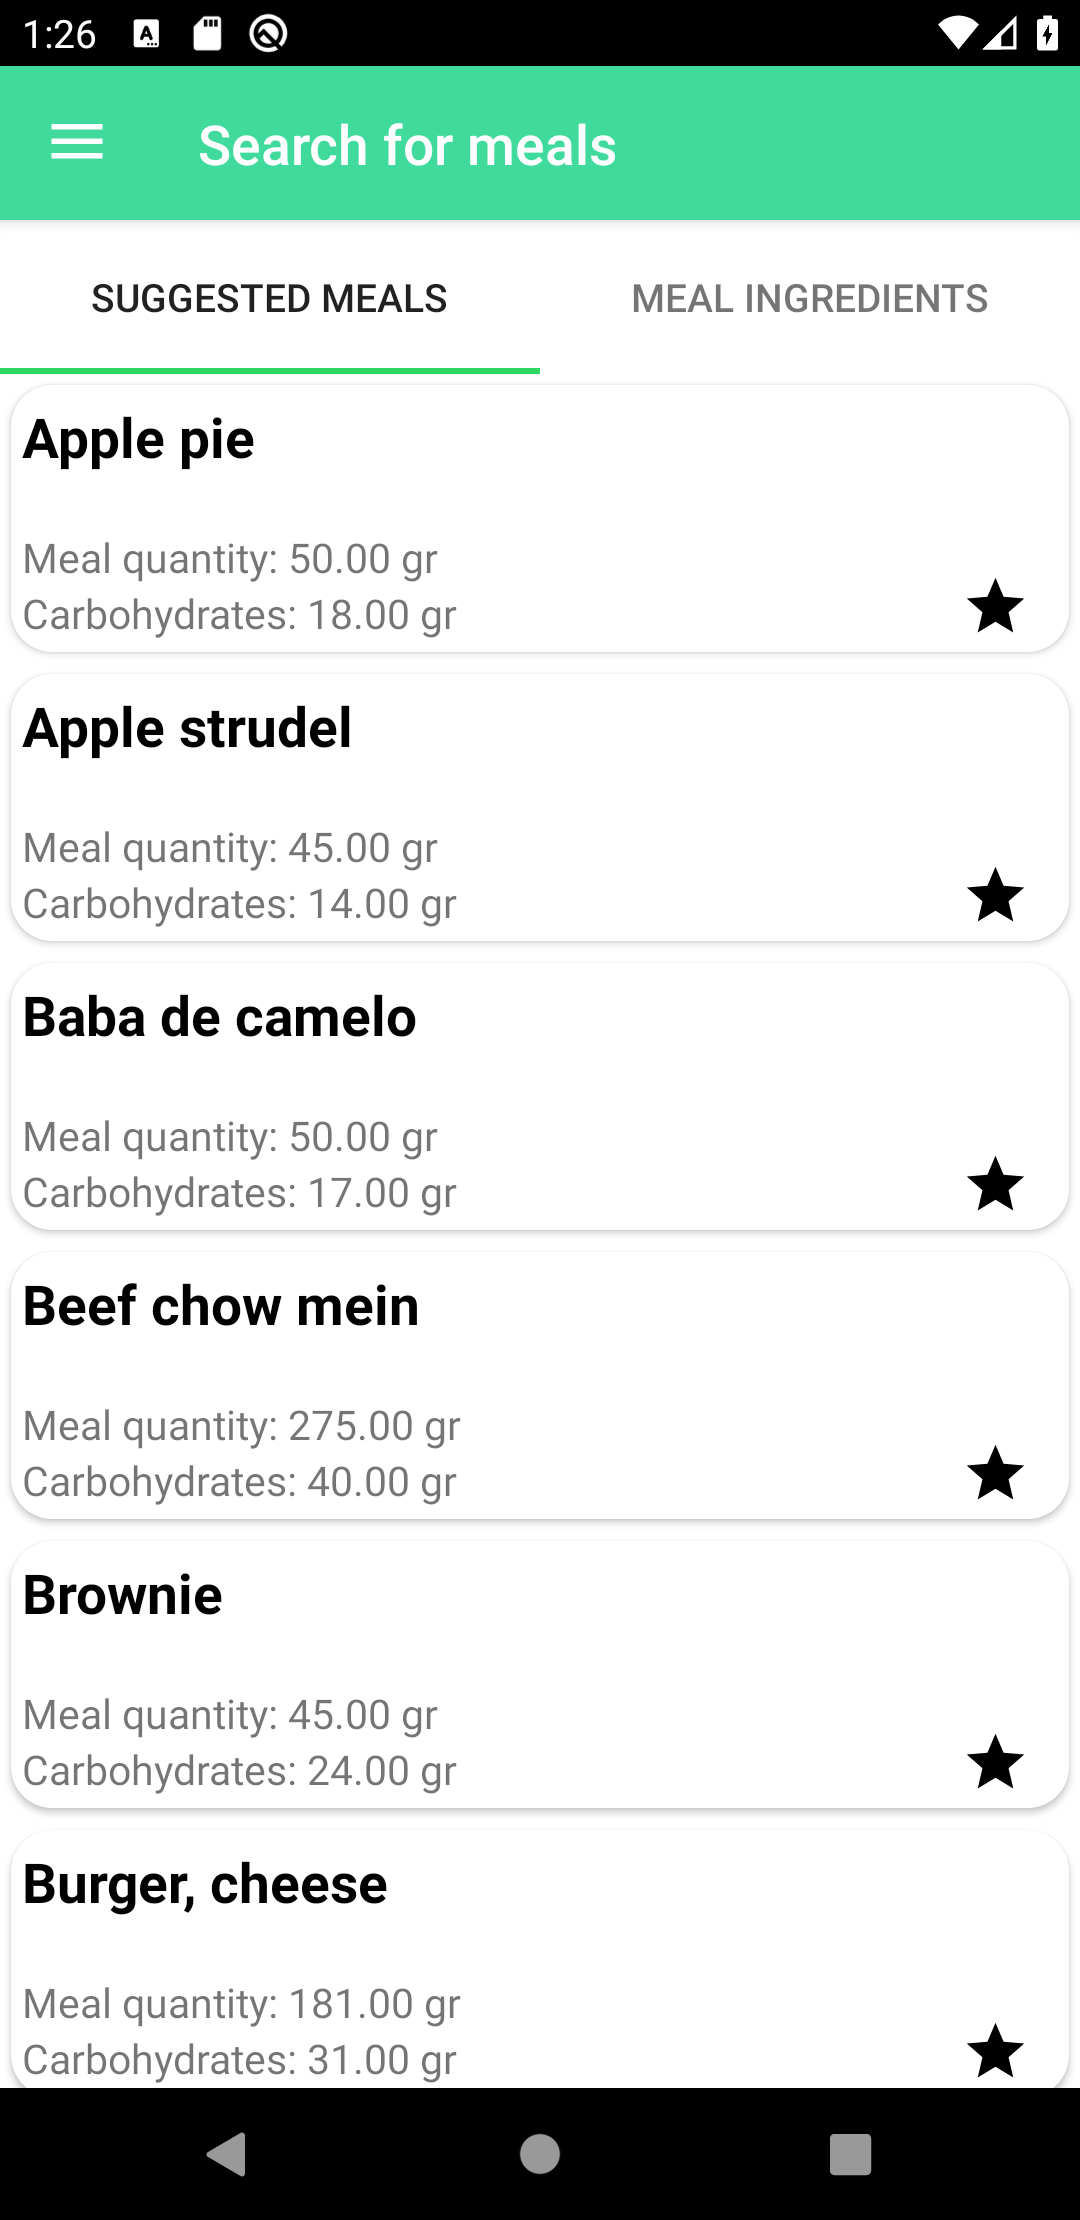
\includegraphics[scale=0.1, width=\textwidth]{_figures/suggested_meals.png}
            \caption{Suggested meals list} 
        \end{subfigure}
        \begin{subfigure}{.3\textwidth}
            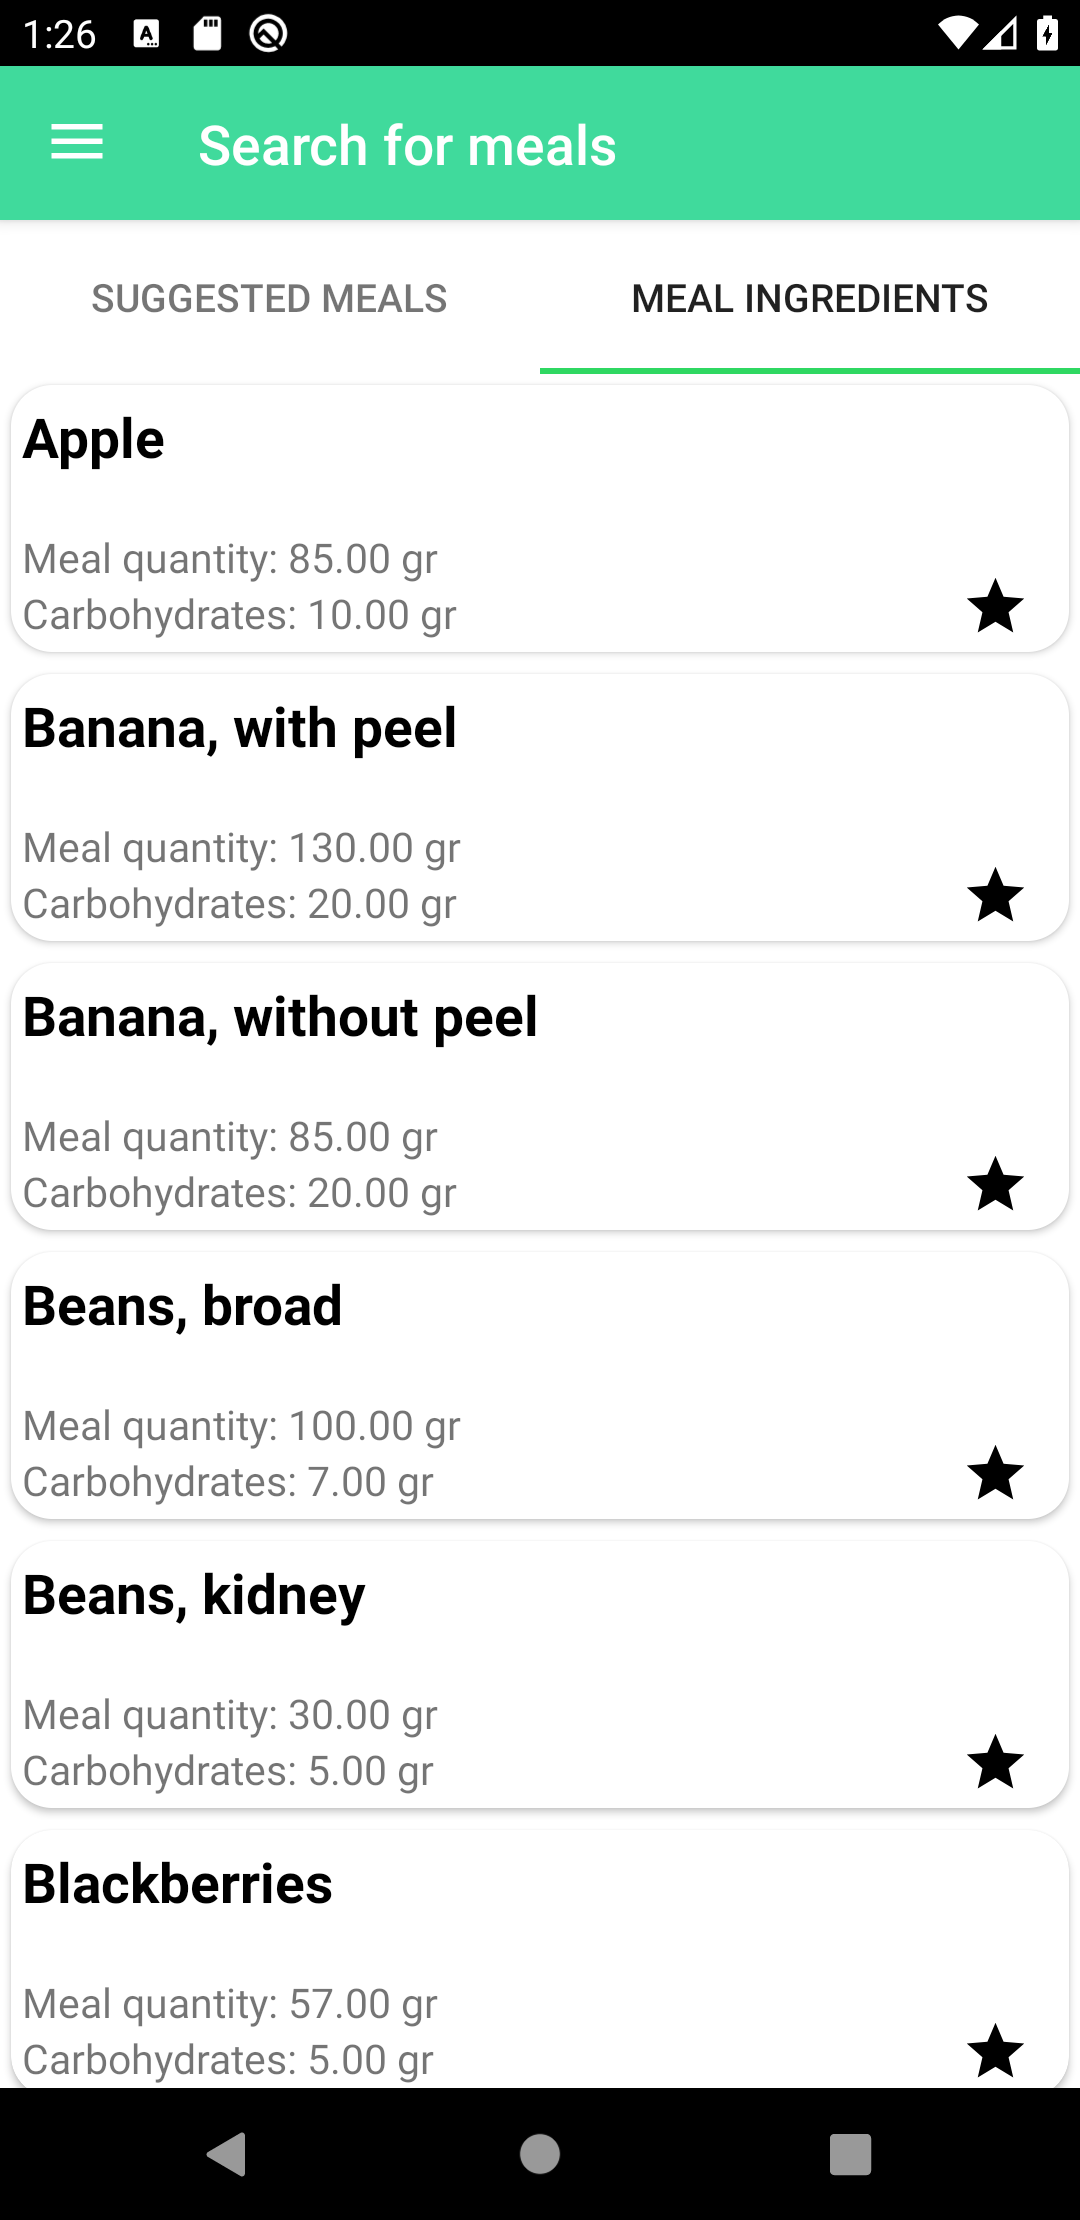
\includegraphics[scale=0.1, width=\textwidth]{_figures/meal_ingredients.png}
            \caption{Meal ingredients list} 
        \end{subfigure}%        
    \end{center}
\end{figure}

\subsubsection{Creating custom meals}

\subsubsection{Using the insulin calculator}

To use this feature, the user must create at least one insulin profile which time period matches the current time. If the user does not have a valid insulin profile for the current
time, the profile information in this fragment will appear with blank fields.\\

\begin{figure}[H]
    \captionsetup[subfigure]{justification=centering}
    \begin{center}
        \begin{subfigure}{.3\textwidth}
            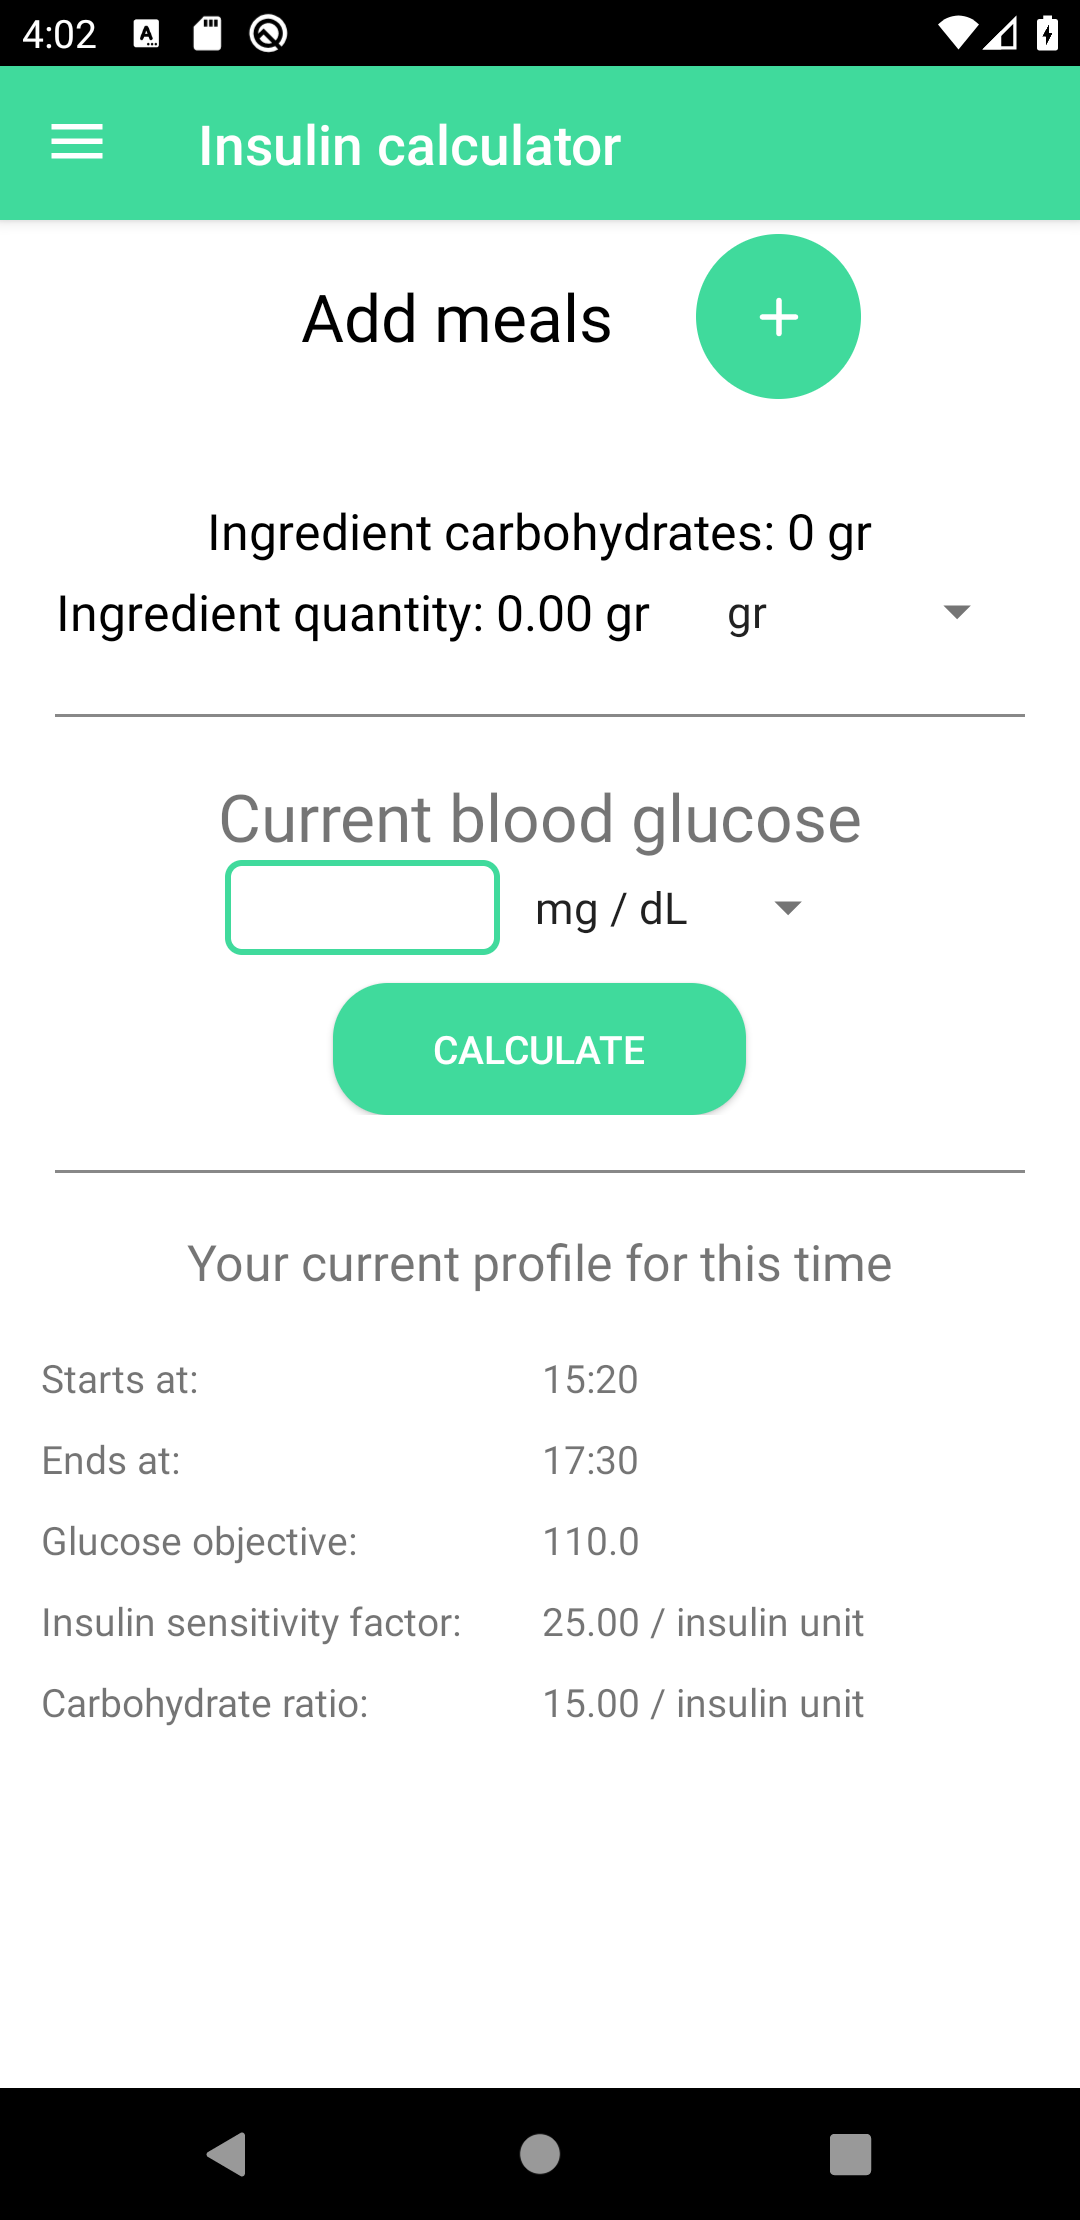
\includegraphics[scale=0.1, width=\textwidth]{_figures/calc_with_profile.png}
            \caption{Calculator with valid profile} 
        \end{subfigure}
        \begin{subfigure}{.3\textwidth}
            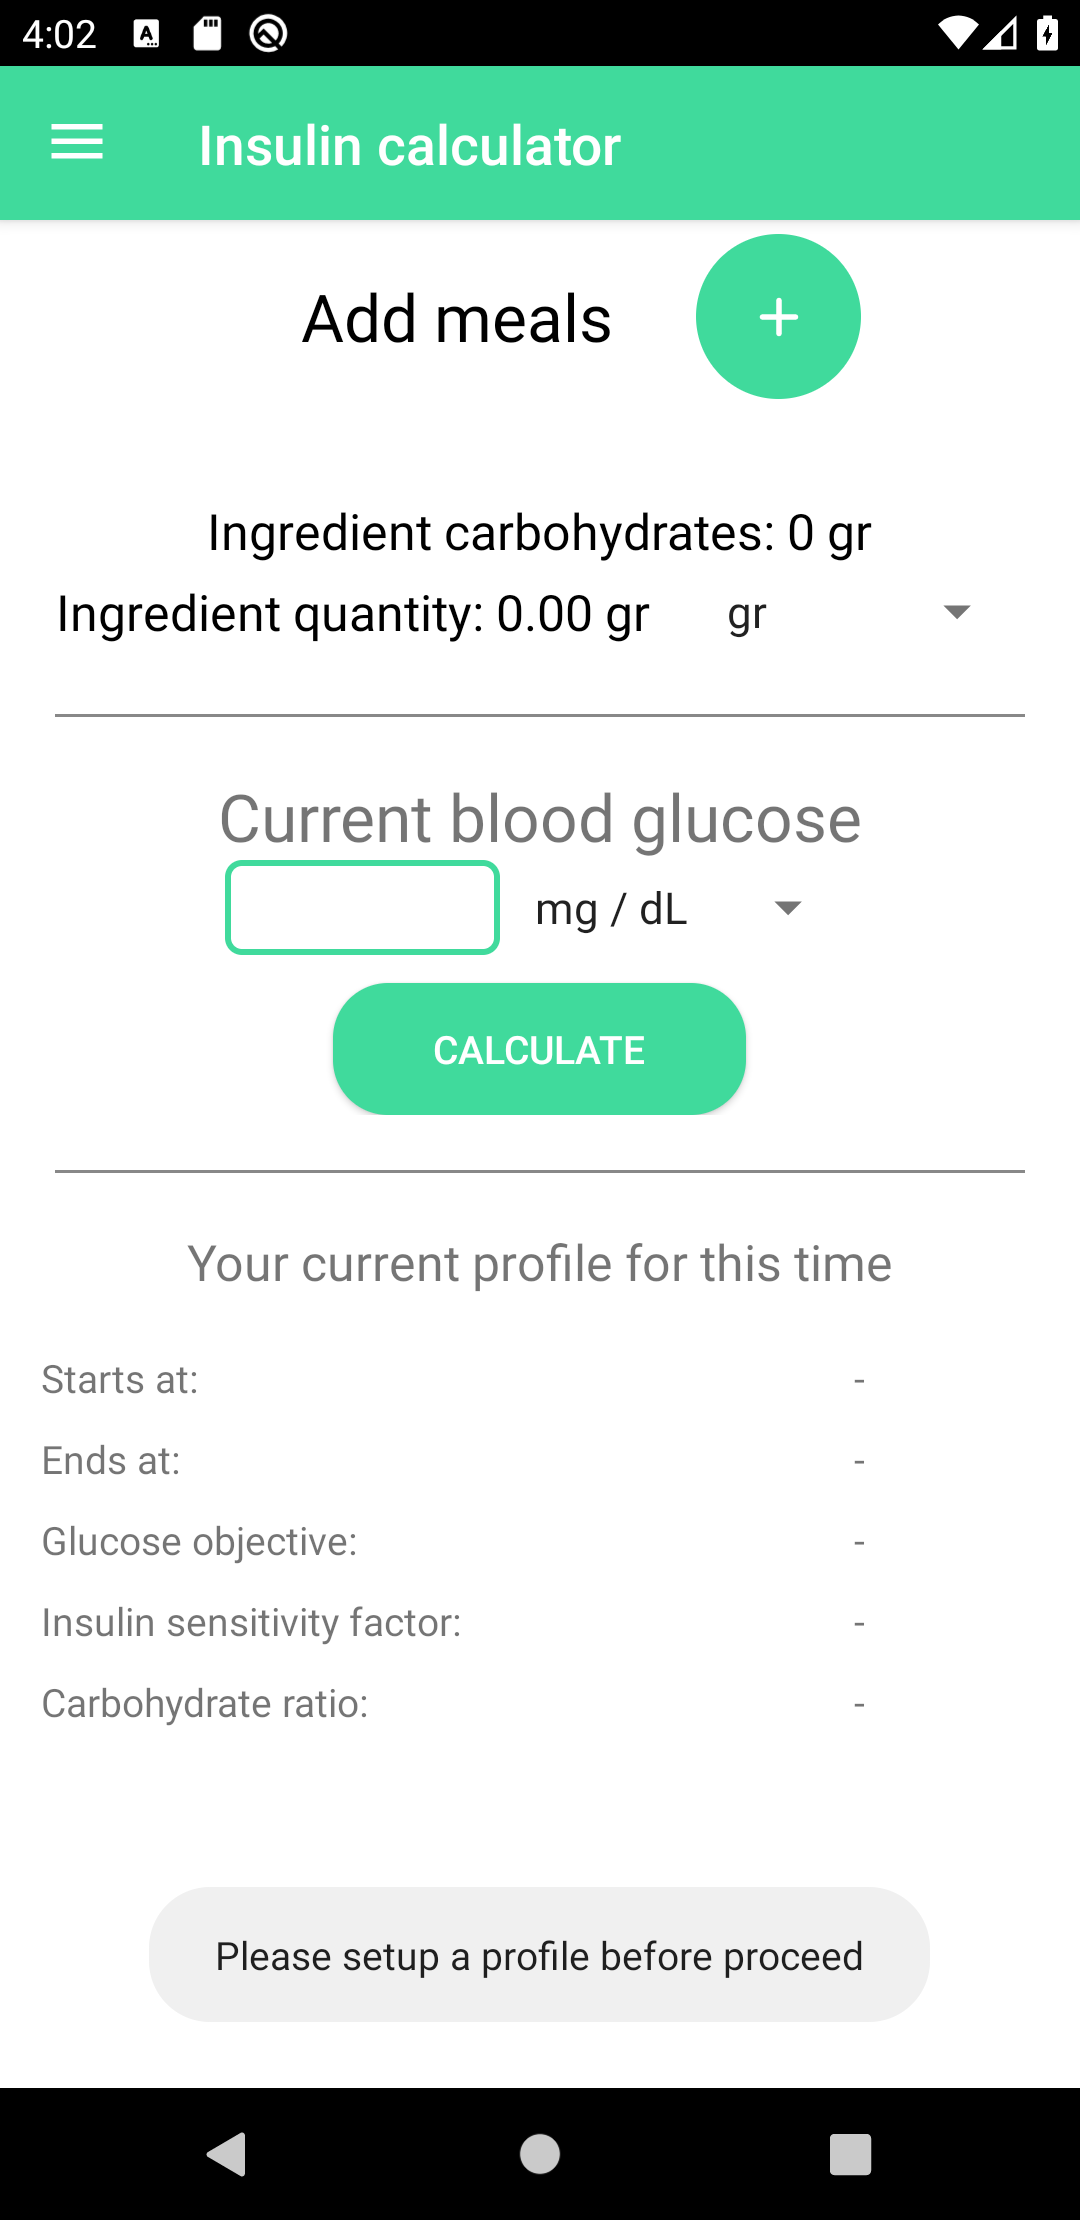
\includegraphics[scale=0.1, width=\textwidth]{_figures/calc_without_profile.png}
            \caption{Calculator without profile} 
        \end{subfigure}%        
    \end{center}
\end{figure}

Having a valid insulin profile, the user must measure its current blood glucose value and select a meal by pressing the plus green button.
When this button is pressed, a tab menu will appear where the user can add:
\begin{itemize}
    \item user's custom meals;
    \item user's favorite meals
    \item ingredients from meals;
    \item suggested meals; 
\end{itemize}

\begin{figure}[H]
    \begin{center}
        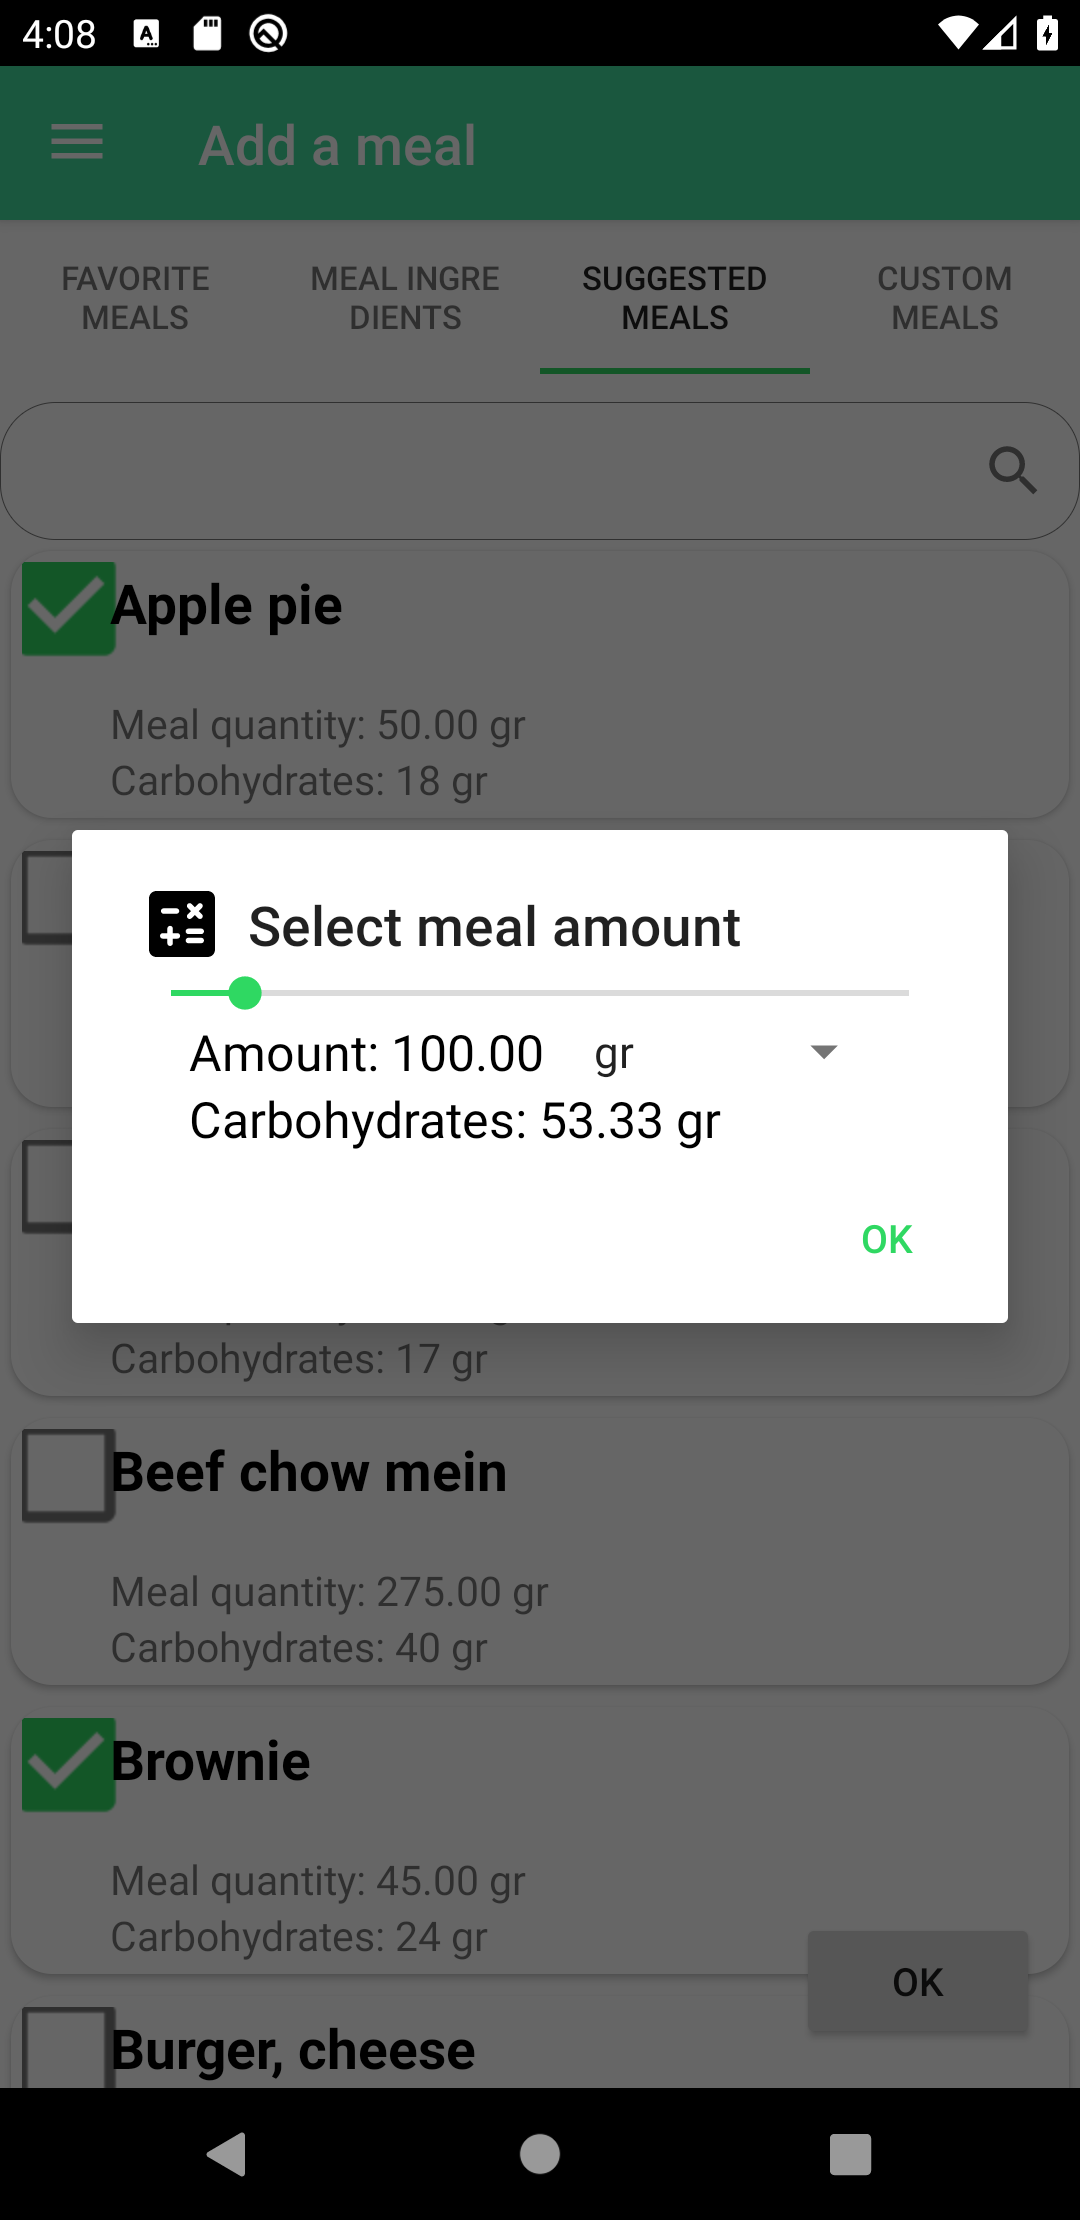
\includegraphics[scale=0.1]{_figures/calc_meal_selection.png}
        \caption{Meal selection menu}
    \end{center}
\end{figure}

After these steps, the user is ready to calculate the insulin dosage that corresponds consuming the select meals, with its current blood glocuse for its current time.

\begin{figure}[H]
    \captionsetup[subfigure]{justification=centering}
    \begin{center}
        \begin{subfigure}{.3\textwidth}
            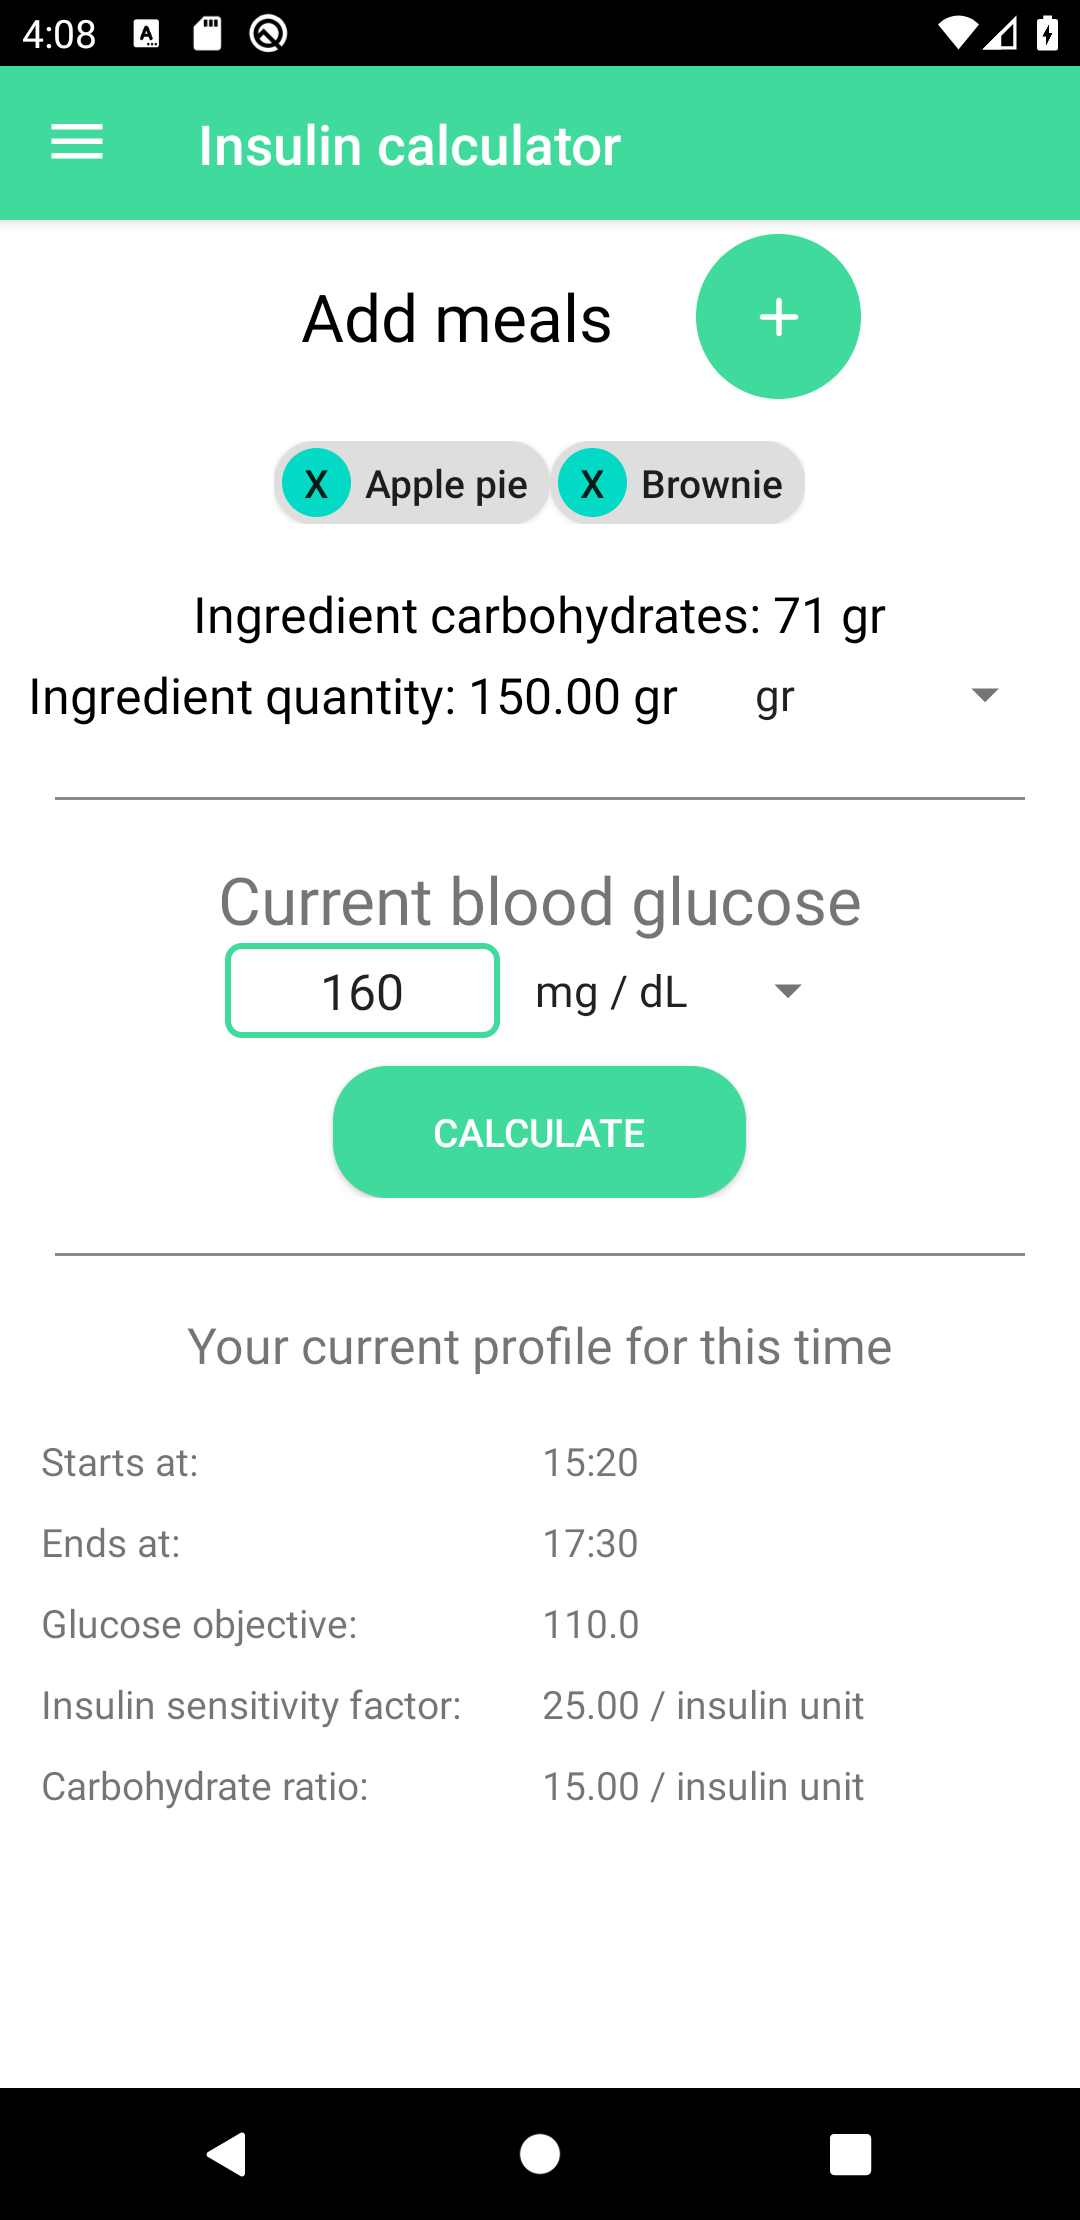
\includegraphics[scale=0.1, width=\textwidth]{_figures/fullfilled_calc.png}
            \caption{Calculator with all the valid field filled} 
        \end{subfigure}
        \begin{subfigure}{.3\textwidth}
            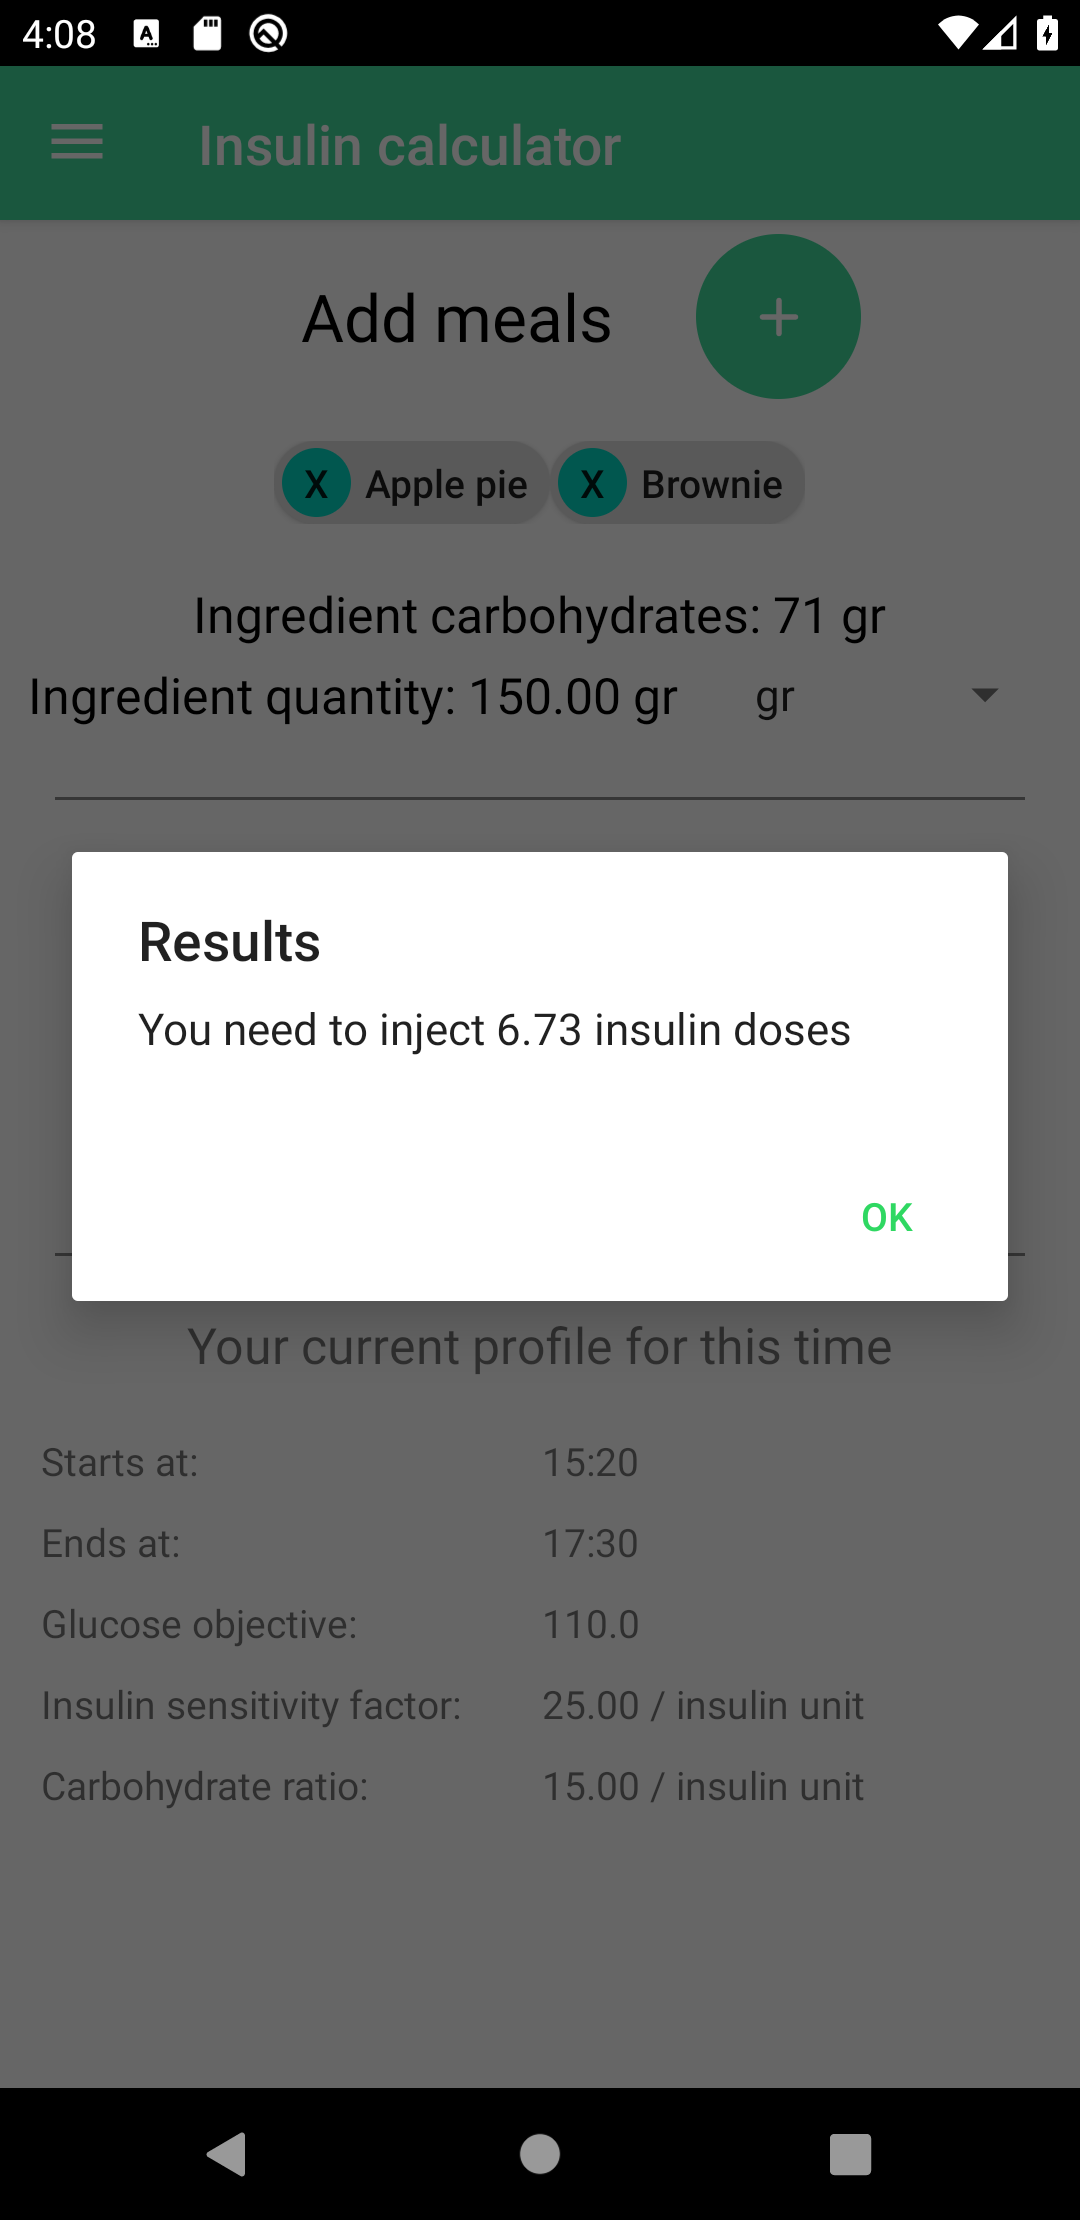
\includegraphics[scale=0.1, width=\textwidth]{_figures/dosage_result.png}
            \caption{Dosage result\\} 
        \end{subfigure}%        
    \end{center}
\end{figure}

\section{Web browser application}

This web browser application will only serve the propose of moderation inside our platform, as we agreed that a good way to provide a good reason for this 
component's existence was to not duplicate the mobile application functionalities and to extend the platform's features.\\

\subsection{Used tecnologies}

\subsubsection{React framework}

We chose to build the website with JavaScript \cite{javascript} using the React framework \cite{react} , as it was the framework lectured in the Web applications
development course and has innumerous advantages to other frameworks, such as Node.JS.

\subsubsection{Bootstrap}

\subsection{Code structure}

\subsubsection{Single-page application}

As website design pattern, we chose to conceive a single-page application. This pattern was chosen for a 
variety of reasons, being the main one a better performance comparing to a traditional multi-page application.\\

\subsubsection{Routing}

As mentioned that the web client application will only serve the propose of moderation, this routing diagram shows the
navigation and routing inside it.

\begin{figure}[H]
    \begin{center}
        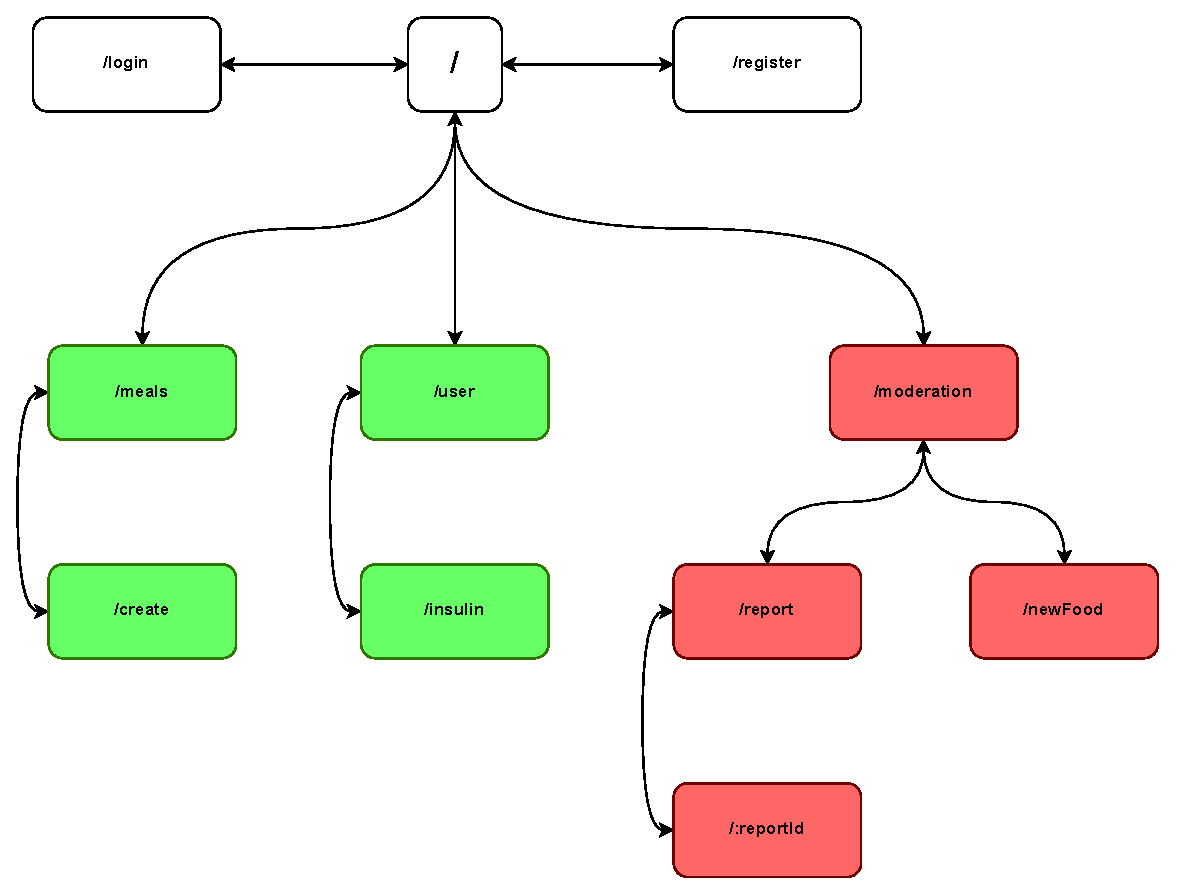
\includegraphics[scale=0.7]{_figures/web-client-endpoints.eps}
        \caption{The web client's navigation diagram}
    \end{center}
\end{figure}

\subsection{Functionalities}

\subsubsection{Register and login}

\begin{figure}[H]
    \begin{center}
        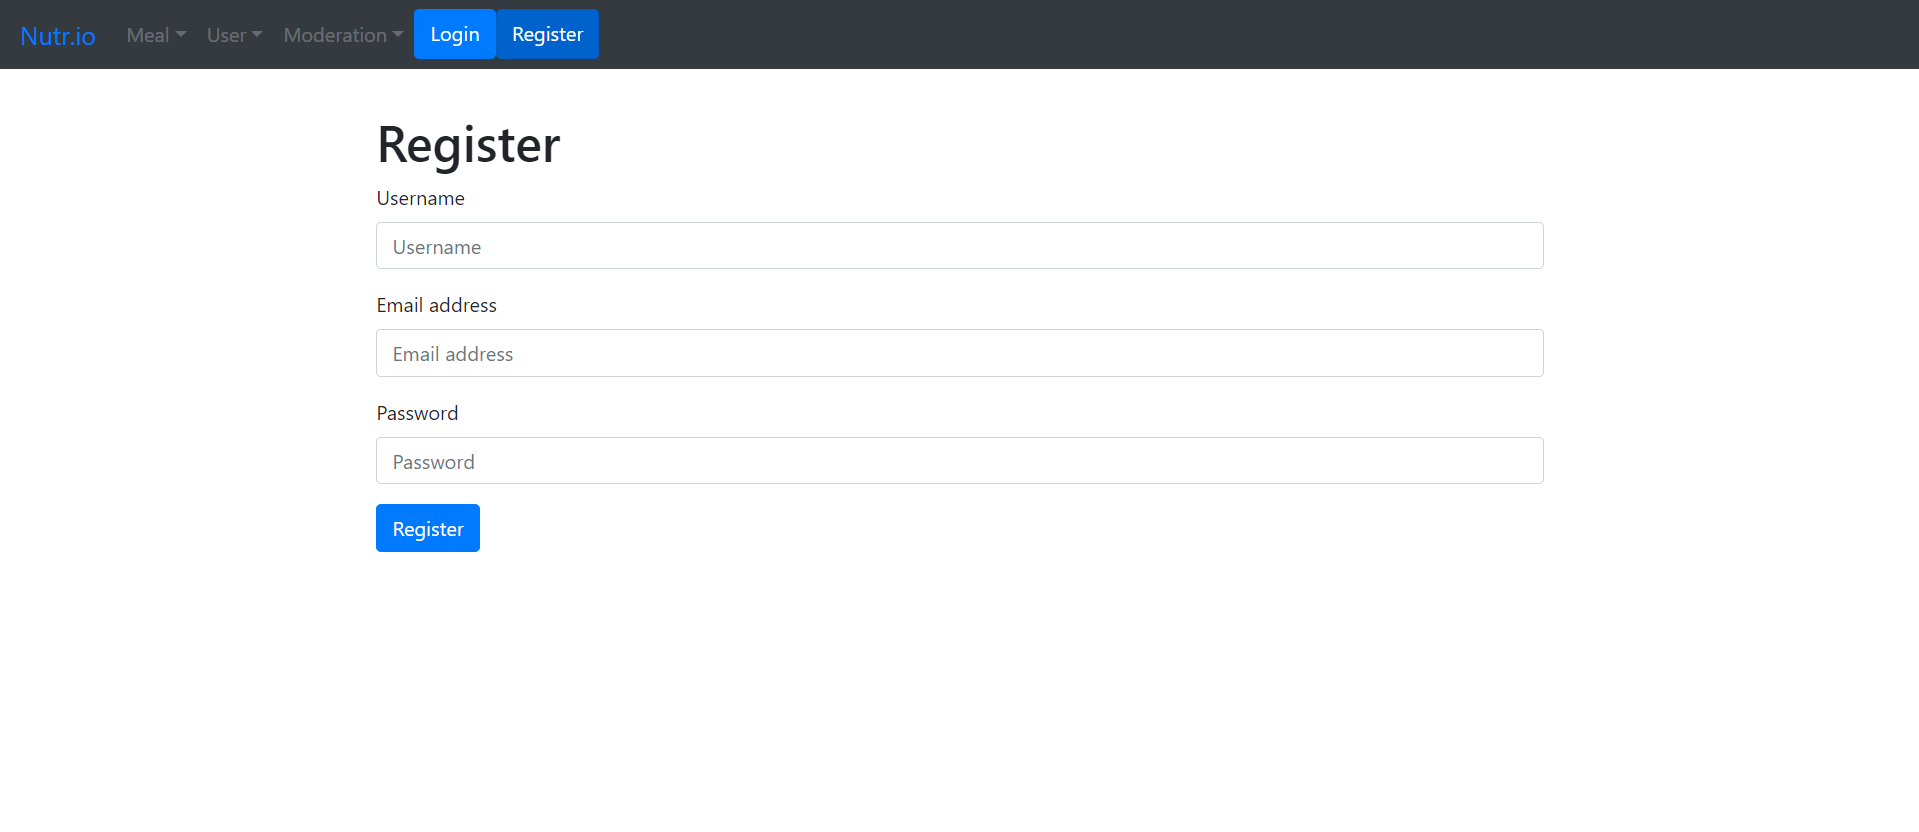
\includegraphics[scale=0.4]{_figures/register-page.png}
        \caption{The register and login page}
    \end{center}
\end{figure}

\subsubsection{Moderator: Create a meal or ingredient}

\begin{figure}[H]
    \begin{center}
        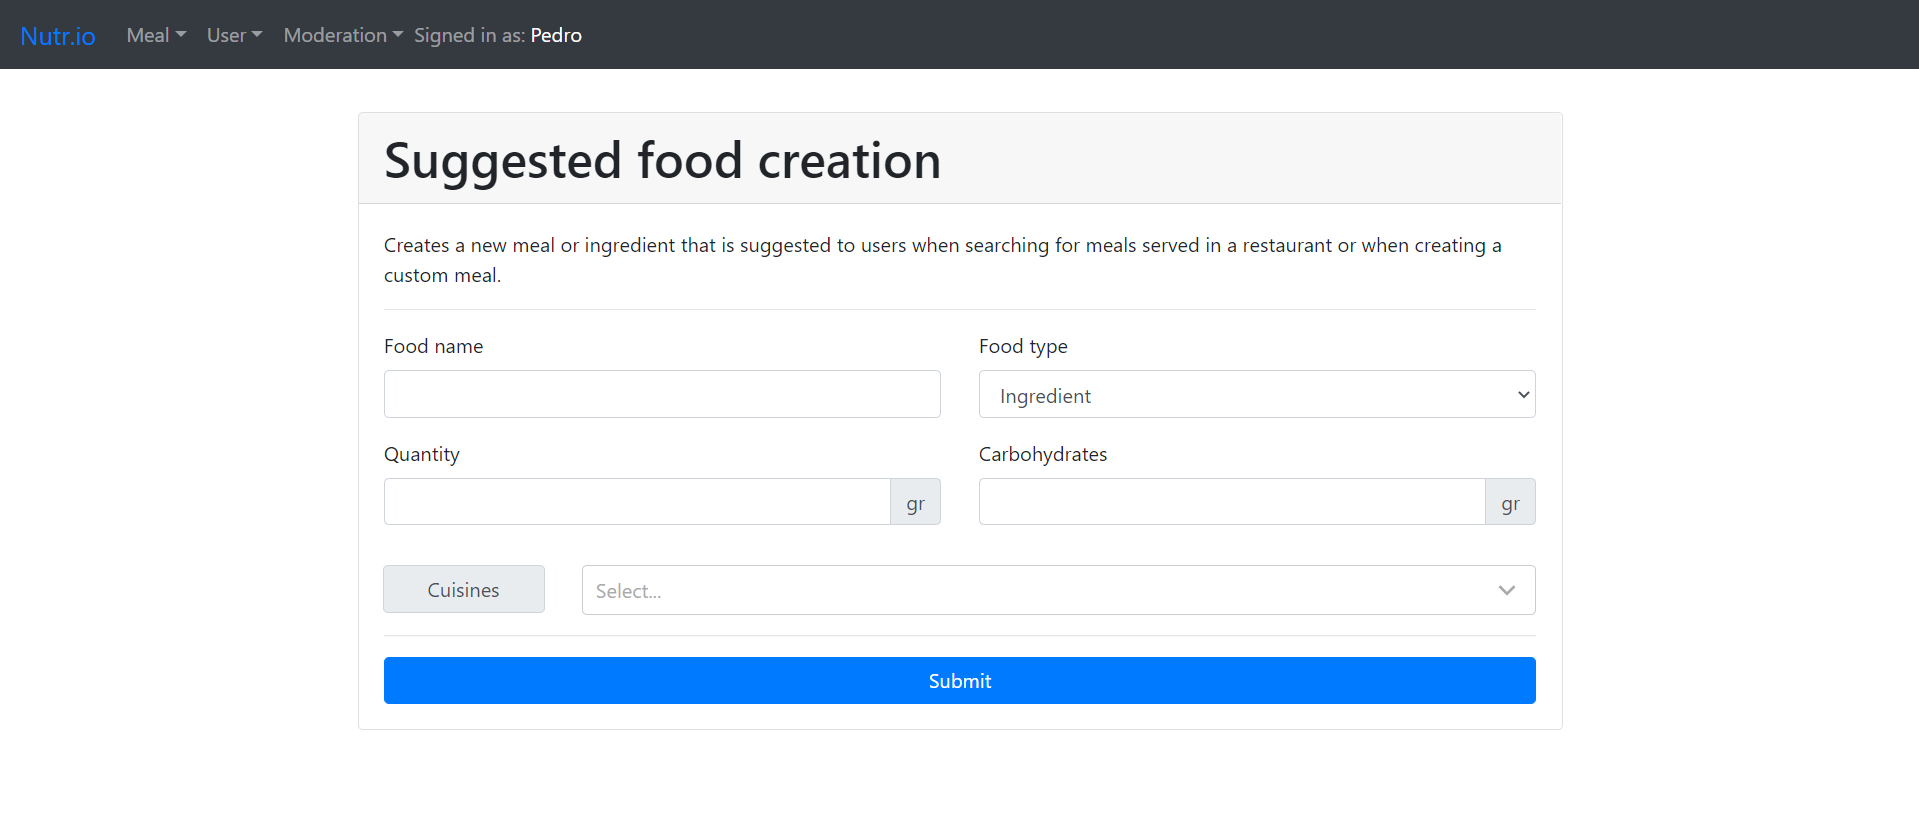
\includegraphics[scale=0.4]{_figures/hardcoded-meal-creation.png}
        \caption{Create a hardcoded meal or ingredient}
    \end{center}
\end{figure}

\subsubsection{User: Create a custom meal}

Meal creation is done in 5 steps and each can only be advanced when all fields are valid
Going back and forth on each step remembers your choices, so editing a previous input is not cumbersome on the user.\\

The sum of all ingredient quantities can not be higher than the original quantity. 
But a meal can always have a leftover quantity which is considered undefined ingredient(s) or ingredients with no carbs.\\

\begin{figure}[H]
    \begin{center}
        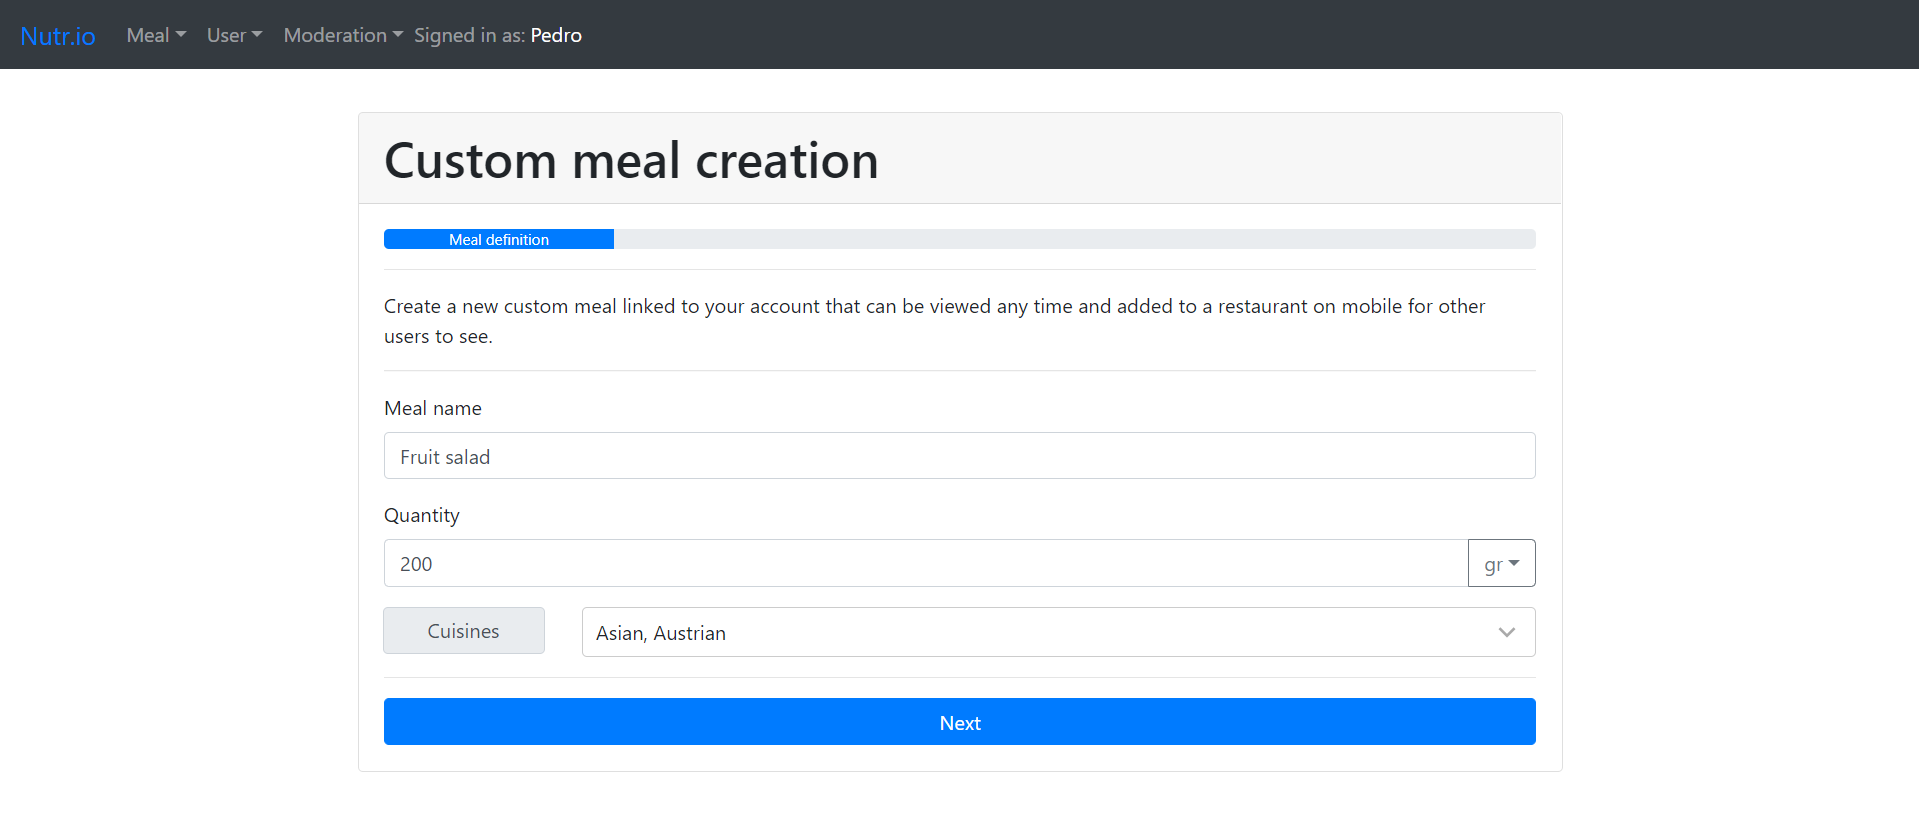
\includegraphics[scale=0.4]{_figures/custom-1.png}
        \caption{Meal description (name, quantity and cuisines)}
    \end{center}
\end{figure}

\begin{figure}[H]
    \begin{center}
        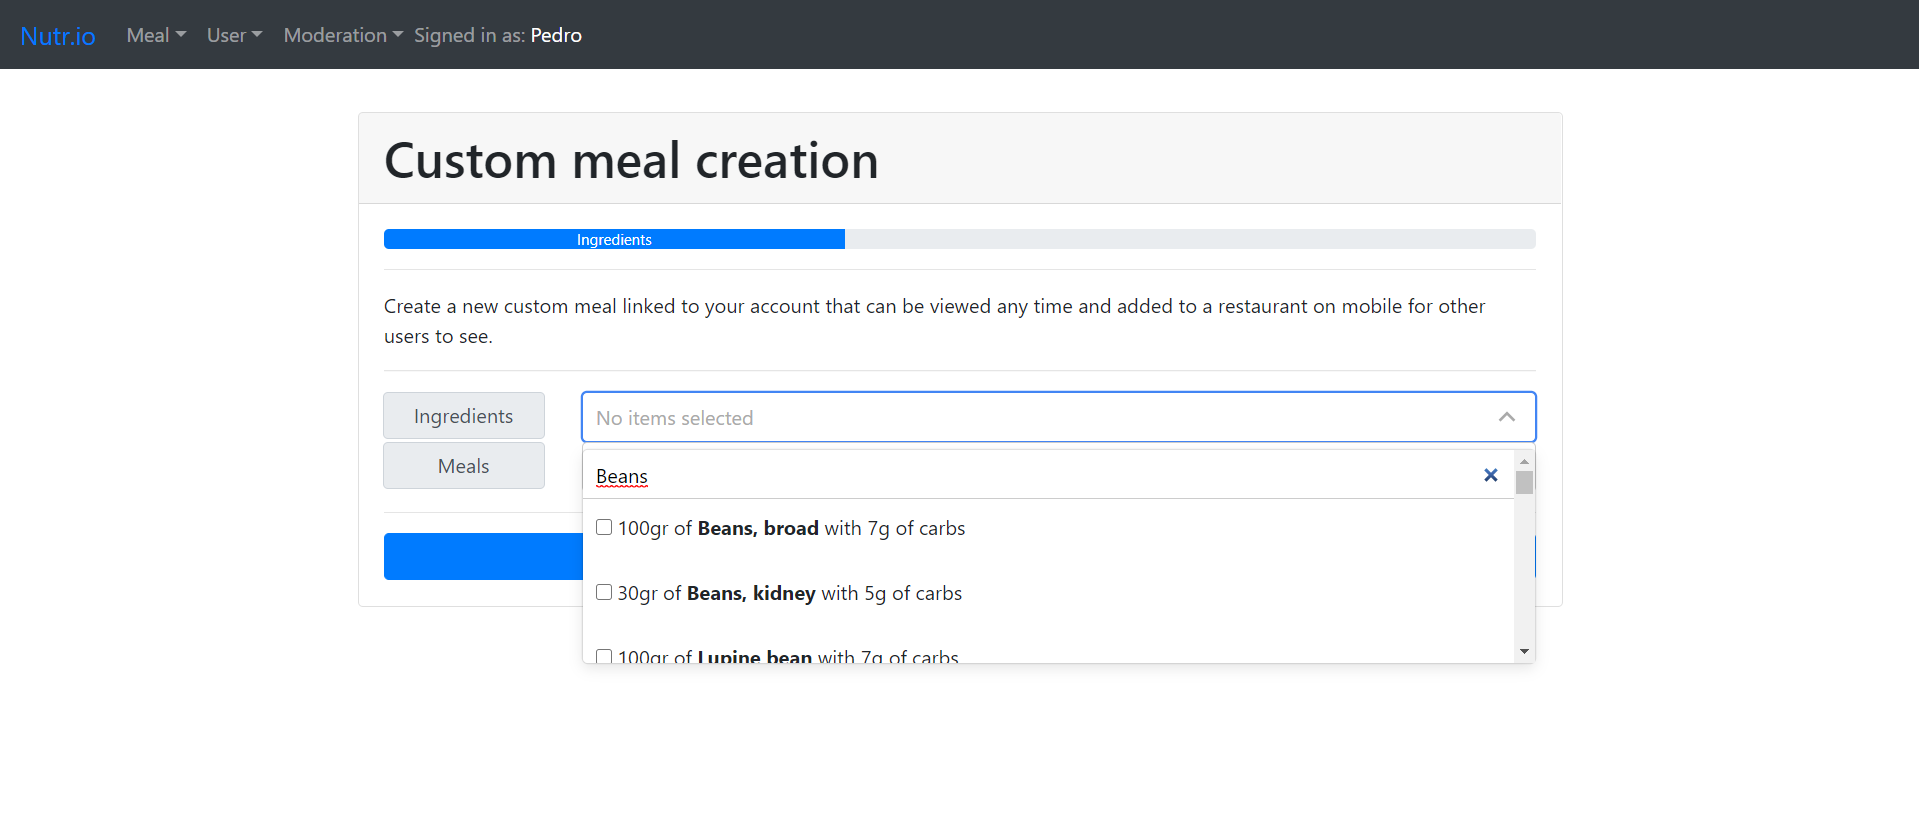
\includegraphics[scale=0.4]{_figures/custom-2.png}
        \caption{Ingredients (in the form of basic ingredients and other complex meals) are chosen}
    \end{center}
\end{figure}

\begin{figure}[H]
    \begin{center}
        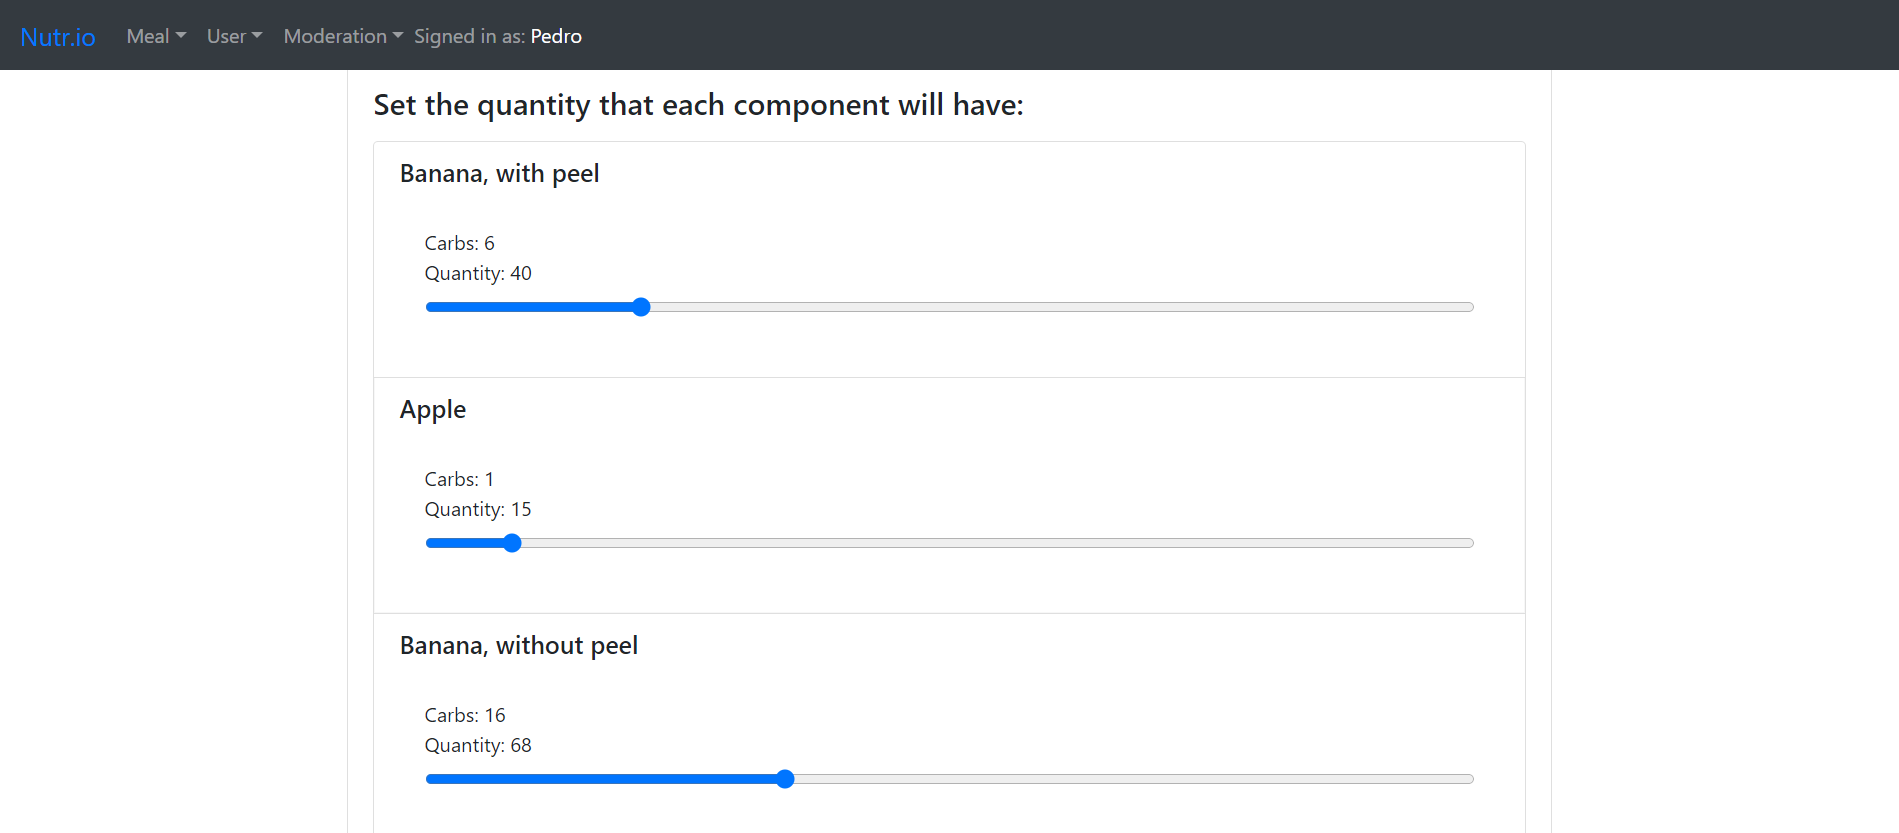
\includegraphics[scale=0.4]{_figures/custom-3.png}
        \caption{User chooses quantity for all chosen ingredients}
    \end{center}
\end{figure}

\begin{figure}[H]
    \begin{center}
        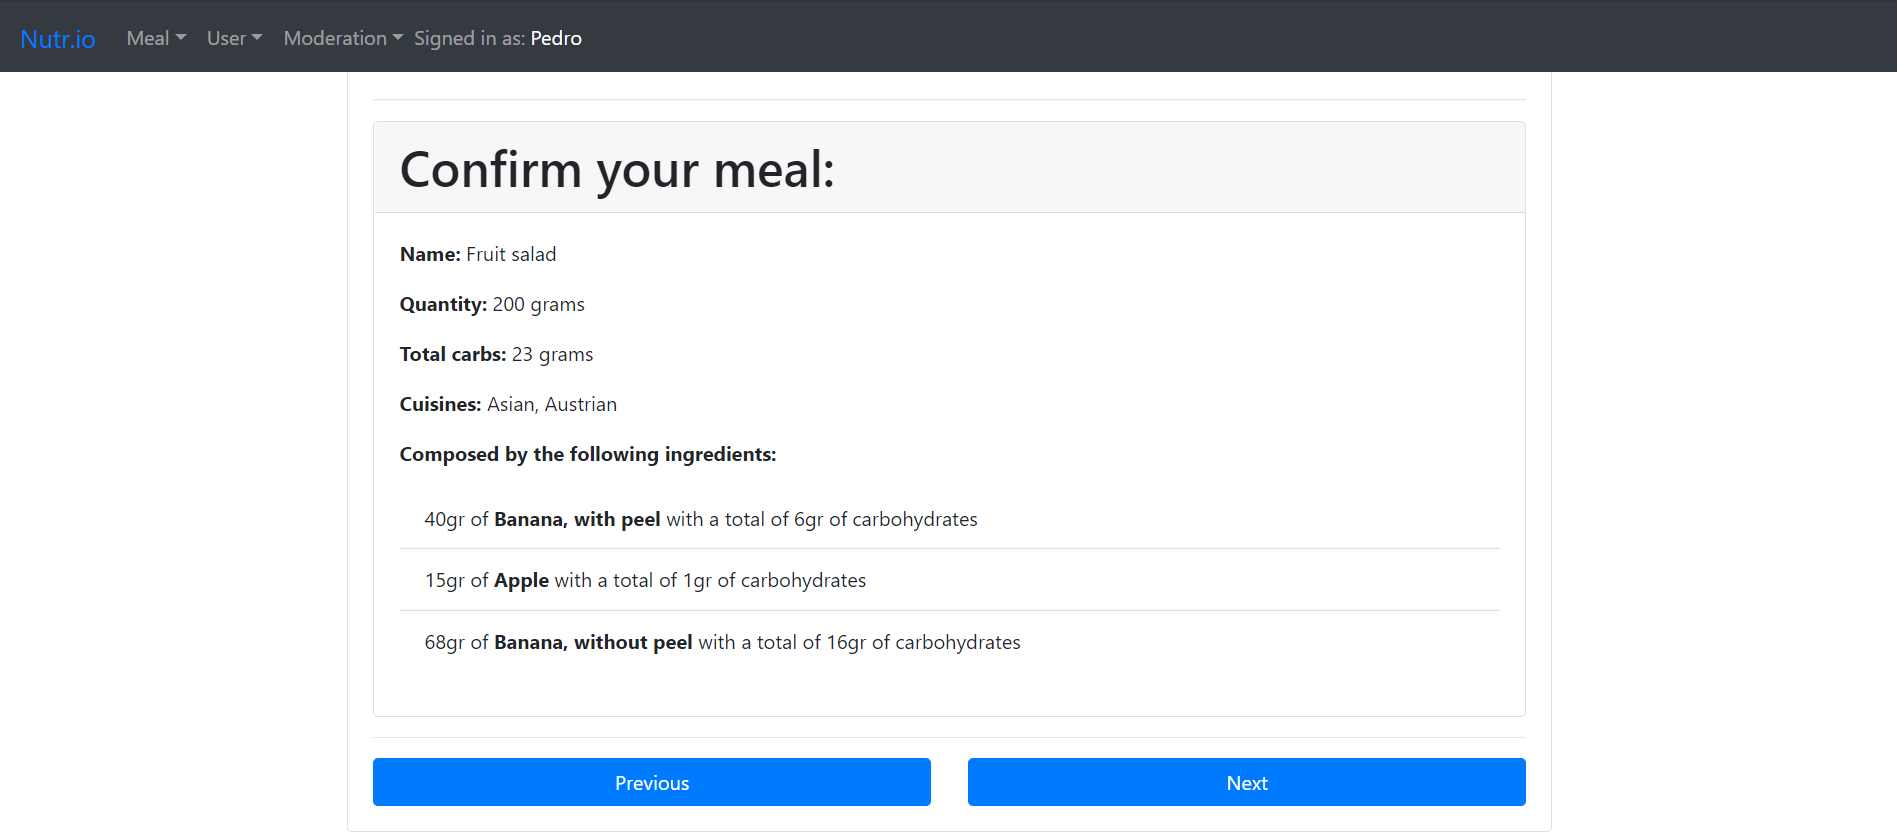
\includegraphics[scale=0.4]{_figures/custom-4.png}
        \caption{Input confirmation}
    \end{center}
\end{figure}

\begin{figure}[H]
    \begin{center}
        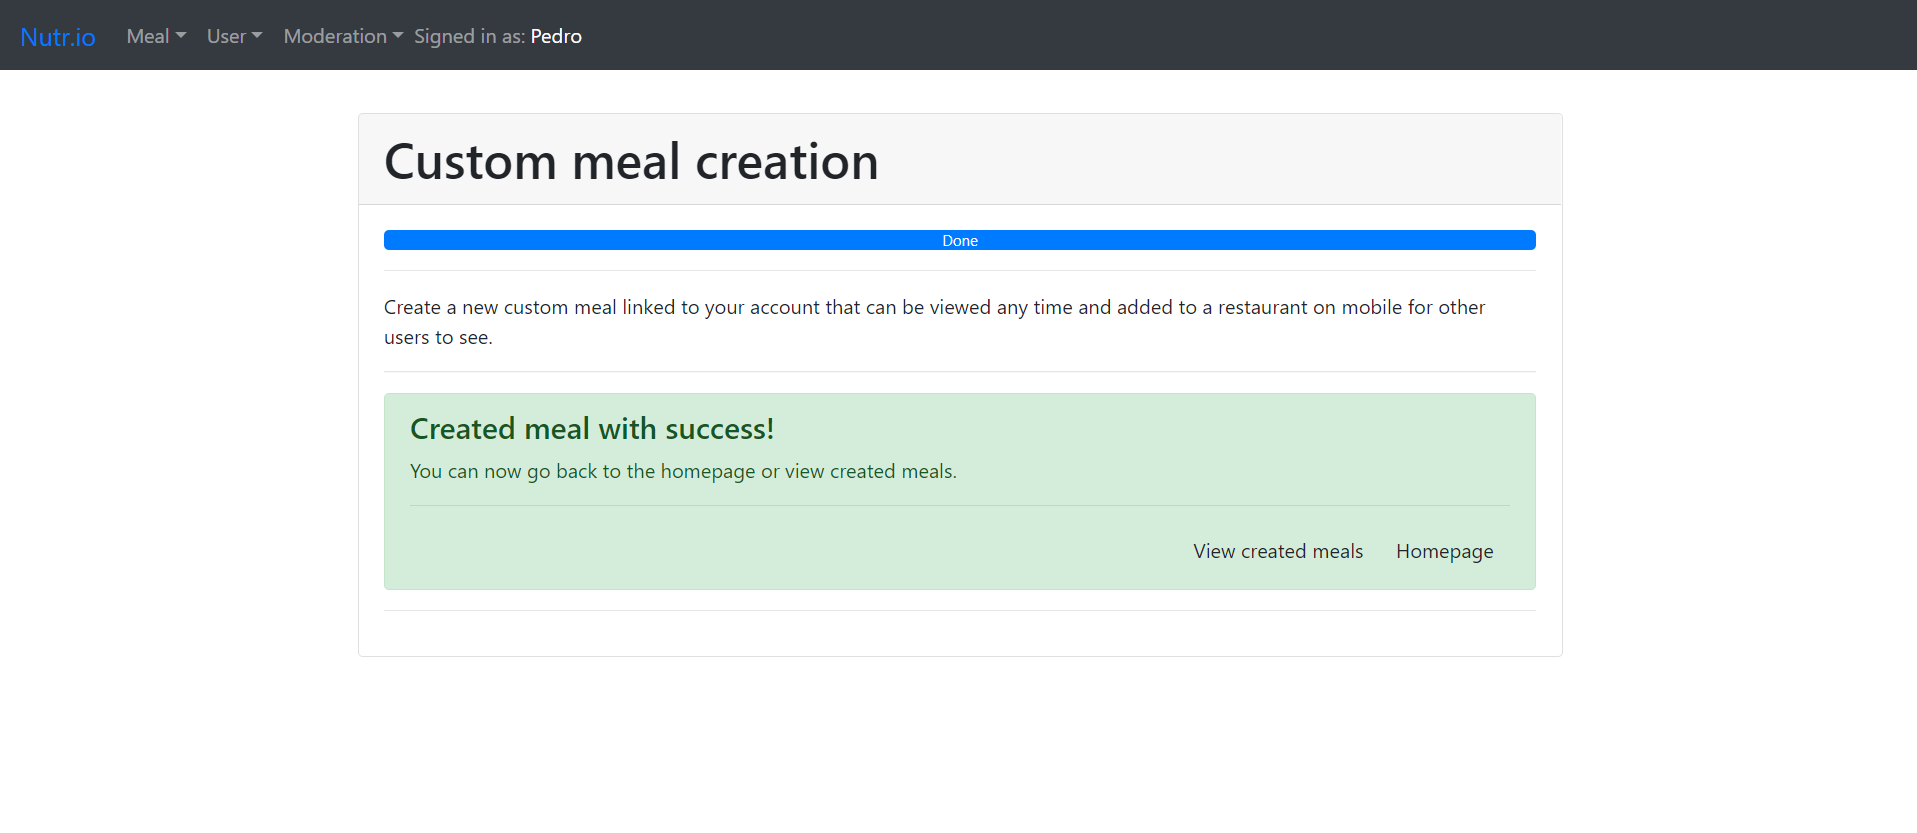
\includegraphics[scale=0.4]{_figures/custom-5.png}
        \caption{Send}
    \end{center}
\end{figure}

\subsubsection{User: Create an insulin profile}

\begin{figure}[H]
    \begin{center}
        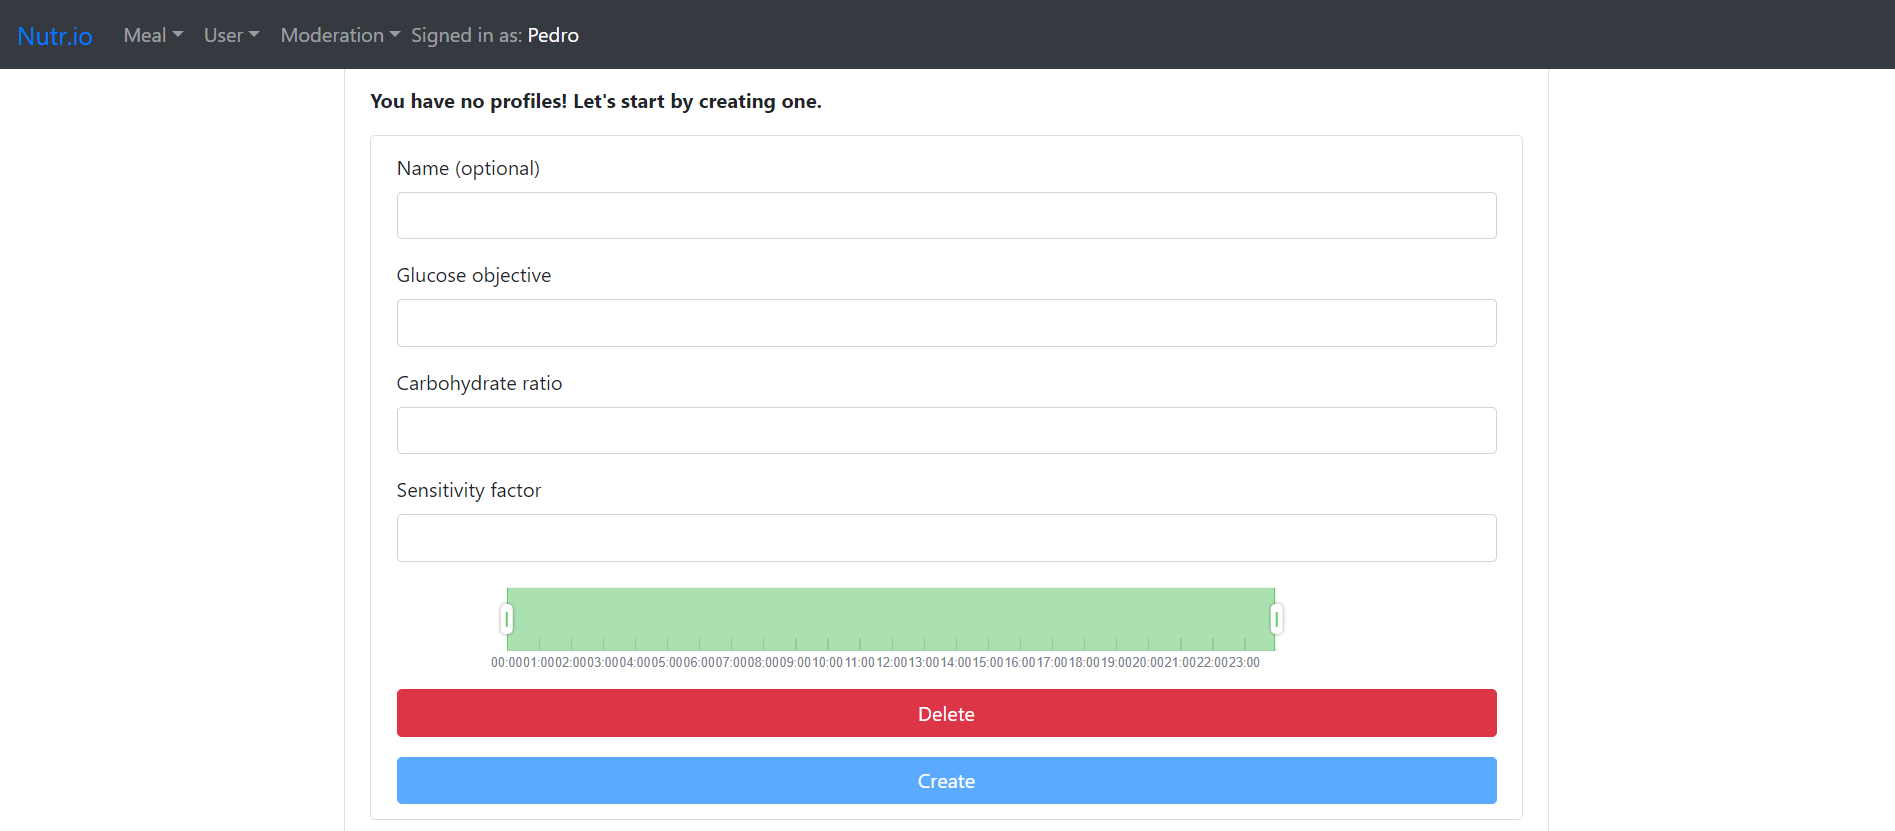
\includegraphics[scale=0.4]{_figures/web-insulin-profile-creation.png}
        \caption{Create a hardcoded meal or ingredient}
    \end{center}
\end{figure}

\subsubsection{Moderator: Consult reports}

\subsubsection{Moderator: Ban users}
